\documentclass[twoside,10pt,a4paper, openright, hidelinks]{extreport}
\usepackage[english]{babel}
\usepackage[T1]{fontenc}
\usepackage{kpfonts}
\usepackage[utf8]{inputenc}
\usepackage{float}
\usepackage[parfill]{parskip}
\usepackage{listings}
\usepackage{setspace}
\usepackage{multicol}
%%\usepackage{calc}
\usepackage{enumerate}
\usepackage{amsmath}
\usepackage{amssymb}
\usepackage{url}
\usepackage{hyperref}
\usepackage{cleveref}
\usepackage{graphicx}
%\usepackage{caption}
\usepackage{subcaption}
\usepackage{natbib}
\usepackage{minitoc}
\usepackage{bibentry}
\usepackage[Lenny]{fncychap}
\usepackage{cases}
\usepackage{fancybox}
%%\usepackage{subfig}
\usepackage{supertabular}
\usepackage{multirow}
\usepackage{blindtext}
%%\usepackage{newtxtext,newtxmath}
\usepackage{rotating}
\usepackage{lscape}
\usepackage{wrapfig}
\usepackage[font={small}]{caption}
\usepackage{array}

% FONT %
%\usepackage[sfdefault]{quattrocento}
%\usepackage[T1]{fontenc}

\usepackage[default,oldstyle,scale=0.95]{opensans} %% Alternatively
%% use the option 'defaultsans' instead of 'default' to replace the
%% sans serif font only.
\usepackage[T1]{fontenc}

\usepackage{wrapfig}

%%%% PAGE DIMENSIONS

%\usepackage[a5paper]{meta-donnees}
%\newcommand{\new}[1]{\textcolor{red}{#1}}
\usepackage[final]{pdfpages}
%\usepackage{meta-donnees}
\usepackage{xspace} 
\usepackage{etoolbox}  % or xpatch
\usepackage{booktabs}
\usepackage[normalem]{ulem}
\useunder{\uline}{\ul}{}
\usepackage{lineno}
\usepackage{placeins}

\usepackage{fancyhdr} %for nice page headers
\fancyhf{}
\fancyfoot{}
\fancyhead[LE,RO]{\small{\thepage}}
\fancyhead[LO]{\nouppercase{\leftmark}}
\fancyhead[RE]{}

%\usepackage[top=1.5cm,bottom=1.5cm,left=1.5cm,right=1.5cm]{geometry}
%\usepackage[papersize={170mm,240mm},top=1.5cm,bottom=1.5cm,left=1.5cm,right=1.5cm]{geometry}
\usepackage{geometry}
\geometry{a4paper} 
\geometry{margin=2.7cm}
\usepackage{pdfpages}

\setlength{\parindent}{0.5cm} % Default is 15pt.
\setlength{\parskip}{0.1 cm}

\usepackage{setspace}

%\linenumbers


%% definition of the encart environnment and associated counter
\newcounter{encartcompteur}[chapter]
\renewcommand{\theencartcompteur}{\arabic{chapter}.\arabic{encartcompteur}}

\newcommand{\encart}[2]{
\refstepcounter{encartcompteur}
\label{box:#1}
%\setlabel{#1}
\begin{wrapfigure}[30]{r}{9cm}
\boxput*(0,1){\colorbox{white}{\textbf{#1}}}{
\setlength
{\fboxsep}{14pt}
\fbox
{\begin{minipage}{8cm}
#2
\end{minipage}}
}
\end{wrapfigure}
}


\newcommand{\encartl}[2]{
\refstepcounter{encartcompteur}
\label{box:#1}
%\setlabel{#1}
\begin{wrapfigure}{l}{9cm}
\boxput*(0,1){\colorbox{white}{\textbf{Box \arabic{chapter}.\arabic{encartcompteur}: #1}}}{
\setlength
{\fboxsep}{14pt}
\fbox
{\begin{minipage}{7cm}
#2
\end{minipage}}
}
\end{wrapfigure}
}


\newcommand{\mwe}{m w.e. a$^{-1}$\xspace}

%\singlespacing
\onehalfspacing
%\doublespacing
%\setstretch{1.1}

%\linespread{1.2}
%\linespread{1.5}


\begin{document}

%\includepdf[pages=-]{D:/01_these/manuscrit/latex_files/couverture/couverture_these.pdf}
\newpage\null\thispagestyle{empty}\setcounter{page}{0}\newpage

\pagestyle{fancy}

\nobibliography*
\pagenumbering{roman}
\dominitoc


%\newpage\null\thispagestyle{empty}\newpage
\vspace*{\stretch{1}}
\begin{flushright}
\begin{small}
\textit{To my parents.}
\end{small}
\end{flushright}

\bigskip
\bigskip

\begin{flushright}
\begin{small}
\textit{To Kadia.}
\end{small}
\end{flushright}
\vspace*{\stretch{2}}
\newpage\null\thispagestyle{empty}\newpage


\section*{Abstract}

The Alps are among the most affected regions in the world by climate change, displaying some of the strongest glacier retreat rates. Long-term interactions between society, mountain ecosystems and glaciers in the region raise important questions on the future evolution of glaciers and their derived environmental and socio-economical  impacts. In order to correctly assess the regional response of glaciers in the French Alps to climate change, there is a need for adequate modelling tools. In this work, we explore new ways to tackle both glacier evolution and glacio-hydrological modelling at a regional scale. Glacier evolution modelling has traditionally been performed using empirical or physical approaches, which are becoming increasingly challenging to optimize with the ever growing amount of available data. Here, we present, to our knowledge, the first effort ever to apply deep learning (i.e. deep artificial neural networks) to simulate the evolution of glaciers. Since both the climate and glacier systems are highly nonlinear, traditional linear mass balance models offer a limited representation of climate-glacier relationships. We show how important nonlinearities in glacier mass balance are captured by deep learning, substantially improving model performance over linear methods. 

This novel method was first applied in a study to reconstruct annual mass balance changes for all glaciers in the French Alps for the 1967-2015 period. Using climate reanalyses, topographical data and glacier inventories, we demonstrate how such an approach can be successfully used to reconstruct large-scale mass balance changes from observations. This study also offered new insights on how glaciers evolved in the French Alps during the last half century, confirming the rather neutral observed mass balance rates in the 1980s and displaying a well-marked acceleration in mass loss from the 2000s on-wards. Important differences between regions are found, with the Mont-Blanc massif presenting the lowest mass loss and the Chablais being the most affected one. Secondly, we applied this modelling framework to simulate the future evolution of all glaciers in the region under multiple (N=29) climate change scenarios. Our estimates indicate that most ice volume in the region will be lost by the end of the 21st century whatever the future climate scenarios. We predict average glacier volume losses of 75\%, 80\% and 88\% under RCP 2.6 (n=3), RCP 4.5 (n=13) and RCP 8.5 (n=13), respectively. By the end of the 21$^{st}$ century the French Alps will be largely ice-free, with glaciers only remaining in the Mont-Blanc and Pelvoux massifs. Our analyses indicate that high-altitude accumulation basins are the most decisive factor determining the future survival of glaciers in the French Alps, followed by higher latitudes. With the warming climate, glaciers retreat to higher elevations in an effort to regain equilibrium with the present climate. Glaciers in high-altitude massifs have a larger altitudinal span to retreat to, offering a colder climate to survive the higher temperatures. In doing so, shrinking glaciers induce major changes in their experienced climate signal, with a reduction in temperature of up to 400 positive degree days (PDD) per year and an increase in snowfall of up to 230 mm per year. We further demonstrate how these complex climate-glacier relationships are highly nonlinear, with linear glacier mass balance models overestimating extreme positive and negative mass balance rates. By taking into account these nonlinear interactions in our model, a largely negative bias in long-term glacier projections was prevented thanks to the nonlinear properties of deep learning. 

This marked glacier retreat in the French Alps will produce an array of consequences that will impact water resources during the warmest months of the year. Glaciers provide cold fresh water resources well after all snow has melted during summer, essential to inhabitants in the region that depend on it for agriculture, industry, ski resorts, hydropower generation and domestic uses. Moreover, several aquatic and terrestrial ecosystems depend on these late summer water resources, that keep water temperature low and ecosystems humid throughout the year. Predicting these changes is of paramount importance in order to correctly anticipate the resulting impacts and to design adequate mitigation strategies. Current hydrological models used in France generally suffer from a simplified representation of glaciers, modelling them as static ice reservoirs. This representation is highly problematic in the current context of rapid glacier retreat. Here, we introduce an updated dynamic representation of glaciers for the J2K hydrological model, validated in a case study in the Arvan partially glacierized catchment. By taking into account the daily area evolution of glaciers, this process-based hydrological model represents an excellent tool to assess the hydrological consequences of glacier retreat at the scale of the French Alps. 
\newpage
%\input{abstract/resume}
%\newpage\null\thispagestyle{empty}\newpage
%\newpage
\section*{Acknowledgements}

This PhD work has been, by all means, a collective effort. I would have never been able to accomplish this without the help, kind words or time from a multitude of people. I am extremely grateful for that, for this project has been an incredible human experience. There are a lot of people that I would like to thank, and I sincerely hope I will not forget anyone. First of all, I would like to thank my parents, for giving me the opportunity and freedom to pursue my studies, which gave me the independence to control my professional career and aim it towards the things I love and matter to me. All of this would not have been possible without Kadia, my closest companion, the hidden co-author, who took care of me during these years despite the long rants on glaciers, climate and machine learning. I am also extremely grateful for the family I have. Laia, Mariona, Andrew, for all the time shared together, especially in New Zealand; and my grandparents, particularly avi Robert, who taught me maths and physics, and who I wish I could show this work. 

Then, I would like to thank my supervisors, who gave me the possibility to do this work, and who always respected my vision and way of working. Antoine, for his availability, dedicating whatever time needed to my problems, and protecting me from several ordeals regarding French paperwork. Being able to discuss in Spanish at the beginning of the PhD was a great way to engage in deep discussions on glaciers, and improved my confidence as a total newcomer to the field. Isabelle, who guided me in the most kind way, and provided invaluable insights on climatology and hydrology, especially during the last hectic weeks of the PhD debugging the hydrological model. I particularly appreciate the freedom I was given to work on the ideas that drive me, knowing the cost that this represented on her research part. For that, I am grateful, but also sorry for not having managed to include them in a better way. Eric and Thomas, who provided insightful comments throughout my work, and whose hydrological expertise helped me during the last part of this work. Special thanks go to Clovis Galiez, who has played the role of a bonus supervisor. I learnt so much about machine learning from him, and our discussions have been to me some of the most stimulating ones during these three years, including several times when his suggestions unlocked problems that I had for weeks. Sven Kralisch has also provided me with guidance on hydrological modelling during the last months. Despite finally not being able to visit Jena, I have always been surprised by his sincere kindness, availability and will to help. 

My PhD companions have proved to be my best allies for such a long journey, with many people I would like to thank. Julien, Joseph, Gabi and Nathan shared with me some of the most memorable adventures on two wheels, from the Alps to Utah. Maria, Gabi, both Juliens, Jai, Jonathan, Joseph and Ambroise shared many hours of skinning up and skiing down snowy mountains, reminding us why we love them so much. Ugo, for the long discussions in the office, attempting to solve the world's problems besides finishing our PhDs, and for the amazing time in Stiappa. Lucas, Olivier and Juan Pedro, for being excellent office partners, and for the stimulating conversations. Romain, Marion, Astrid, Amber, Diego, Hans, Foteini, Isabelle, Albane, Sammy, Jinwha, Laura, Pedro, Peter, Sarah, Claudio, Maxim, Fanny and Marco, for the great times shared in the lab, in conferences, in the mountains or at the bar. I acknowledge the long term help and support from Molts Ànims, my good old friends in Sant Cugat, who have always been there and who always make me feel home despite the long seven years living abroad. And particularly Edu, who besides sharing almost all the university years with me, provided me with lots of insight on machine learning at the beginning of my PhD.

I am also grateful to Delphine, Olivier and Bruno, who taught me how to measure glacier mass balance in the field, in some of the most breathtaking landscapes I have ever seen. I had so much fun doing that, but I will particularly remember the day when, together with Delphine, we measured all the ablation stakes in Mer de Glace in one long and arduous push. I am especially thankful to the members of my PhD jury for accepting to review this work. I have been lucky enough to have exactly the jury I wished for, and I really appreciate the time and effort that it involves. Moreover, I would also like to thank Christian, Thomas and Agnès, for taking part in my thesis committee, and guiding me with insightful comments  and making it feel more like a conversation than an evaluation. There are many people in the lab(s) that I would also like to thank, for the friendly and interesting conversations in the cafeteria and for the shared small talk: Jérémie, Nico, Sophie, Patrick, Jean-Manu, Gilles, Martin, Manon, Lionel and Vincent. 

Finally, I am grateful for the many scientific interactions I had outside the lab, particularly during conferences and paper reviews. I would like to thank Fabien Maussion, Ben Marzeion and Matthias Huss, who besides being an inspiration to me, provided constructive feedback that truly managed to improve my work. I can only hope to have the same luck with reviewers in the future. I am also very thankful to Daniel Farinotti, who always showed kind interest in my work from the beginning, and who is currently helping me to pursue my scientific ideas for a postdoc. I had the chance to meet Fernando Pérez in San Francisco last year, resulting in stimulating discussions on scientific modelling. I hope we will be able to collaborate in the future, once the currently troubled times calm down. I have very fond memories of my winter school in Mendoza, Argentina. I learnt a lot from Lucas Ruiz, Pierre Pitte, Lidia Ferri, Laura Zalazar, Maxi Viale and Mariano Masiokas, and I met some lovely people with whom I experienced the beauty of the Andes. I also had the pleasure to be part of the NASA ICESat-2 Hackweek, which despite having a virtual format, allowed me to learn from, interact and collaborate with great people from all around the world. At last, I am also thankful for the discussions and feedback from Harry Zekollari for my latest paper, with whom I share very similar research interests and the pleasure of writing long e-mails with lots of figures.

I acknowledge the funding of my PhD work by INRAE, the Labex OSUG@2020 (Investissement d'Avenir, ANR ANR10 LABX56), the Auvergne-Rhône-Alpes region through the BERGER project, the VIP Mont-Blanc project (ANR-14 CE03-0006-03) and the CNES (KALEIDOS-Alpes and ISIS projects grants).

I like to believe that these three years have been a small taste of what science is about: a diverse, inclusive, open and collective discussion on the investigation and discovery of nature. 

\bigskip
\bigskip
\bigskip
\bigskip

\begin{flushright}
\begin{small}
\textit{This manuscript has mostly been written and assembled in the beautiful small village of Stiappa, Tuscany (Italy).}
\end{small}
\end{flushright}

\tableofcontents
%\newpage\null\thispagestyle{empty}\newpage

\pagenumbering{arabic}

\chapter{Introduction}
\label{chap:intro}

\begin{flushright}
\begin{small}
\textit{Even in science, the object of research is no longer nature itself, but man's investigation of nature.}\\
Werner Heisenberg
\end{small}
\end{flushright}

\section{On the importance of glaciers}

Glaciers are fascinating natural systems to study. Their beauty is the consequence of complex interactions between climate and topography, creating  unique natural features that shape landscapes, ecosystems and even climates wherever they flow. These perennial ice masses originate in places allowing the accumulation of snow, that over the course of years gradually transform into firn and eventually ice. Due to gravity, this ice flows downwards, reaching lower elevations with higher temperatures where ice is lost through different processes of ablation, such as ice melting or calving \citep{ipcc_climate_2018}. The sum of all accumulation and ablation in a glacier determines its mass balance, which is essential to track the evolution of glaciers through time and their contribution to sea level rise (Fig. \ref{intro:fig1}). Glaciers are excellent climate proxies, adjusting their geometry and size to changes in climate. They represent a large part of the cryosphere, storing about 69\% of the world's fresh water. In their study, glaciers are often divided into mountain glaciers (Fig. \ref{intro:fig1}) and ice-sheets, which differ in size and geographical location, with ice-sheets being much larger than mountain glaciers and situated in Greenland and Antarctica \citep{benn_glaciers_2014}. 

Mountains are the water towers of the world, acting as buffers that store solid precipitation and distribute fresh water resources throughout the year \citep{immerzeel_importance_2020}. Glaciers play a major role in this, providing water resources during the warmest months well after all snow has melted. This late summer run-off is essential to many ecosystems and about 10\% of the global human population that live in mountain areas and the contiguous plains \citep{huss_global-scale_2018, cauvy-fraunie_global_2019,farinotti_large_2019}. Mountain areas are amongst the most affected regions by anthropogenic climate change, outpacing global warming  with an increase of 0.3ºC per decade \cite{ipcc_climate_2018}. These rapid changes in climate are causing a widespread retreat of glaciers (Fig. \ref{intro:fig1}), with many regions already having reached "peak water", i.e. the maximum in annual glacier run-off. Once this point is reached, glaciers progressively reduce their water contributions, altering the hydrological regime of watersheds \citep{huss_global-scale_2018}. The disappearance of glaciers produces an early release of accumulated precipitation in spring and early summer, with potential droughts in late summer \citep{brunner_future_2019}. These fast changes in mountain glaciers result in glaciers currently being important contributors to sea level rise (0.92 $\pm$ 0.39 mm a$^{-1}$), as much as the massive Antarctic and Greenland ice-sheets combined, despite representing less than 1\% of the ice on Earth \citep{zemp_global_2019, hock_glaciermip_2019}. 

\begin{figure*}[h]
\centering
\includegraphics[width=14cm]{Figures/intro/Figure_1.png}
\caption{Glacier mass budgets for eleven different mountain regions and their combined results. Regional time series of annual mass change are based on glaciological and geodetic balances (Zemp et al., 2019). Superimposed are multi-year averages by Wouters et al. (2019) based on the Gravity Recovery and Climate Experiment (GRACE), only shown for the regions with glacier area >3,000 km2. Estimates by Gardner et al. (2013) were used in the IPCC 5th Assessment Report (AR5). Annual and time-averaged mass-budget estimates include the errors reported in each study. Glacier areas (A) and volumes (V) are based on RGI Consortium (2017)
and Farinotti et al. (2019), respectively. Red and blue bars on map refer to regional budgets averaged over the period 2006–2015 in units of kg m$^{–2}$ yr$^{–1}$ and mm sea level equivalent (SLE) yr$^{–1}$, respectively, and are derived from each region’s available mass-balance estimates. \textit{Figure from IPCC's Special Report on the Ocean and Cryosphere in a Changing Climate (SROCC, 2019).}} 
\label{intro:fig1}
\end{figure*}

Mountain glaciers are predicted to lose an important fraction of their overall mass by the end of the 21$^{st}$ century, with great differences between regions \citep{hock_glaciermip_2019}. The correct assessment of future glacier evolution is essential to understand and quantify the environmental and social consequences of their retreat. Since glaciers have become an icon of climate change, accurate predictions paired with effective communication can prove a great way to raise awareness on climate change. Despite scientific efforts to precisely quantify and understand glacier retreat, the main driver of future uncertainty in predictions are anthropogenic greenhouse emissions \citep{marzeion_partitioning_2020}. Scientific studies on glaciers must find their way into a wider audience in order to effectively contribute to their conservation. By combining an improved understanding of glacier processes with targeted communication of relevant results, we can aim at preserving our own very subject of study.  

\section{Glaciers in the French Alps}

\begin{wrapfigure}{R}{0.55\linewidth}
\centering
\includegraphics[width=8.3cm]{Figures/intro/Figure_2.pdf}
\caption{Glacierized massifs in the French Alps, with the extent of glaciers for the year 2015.}
\label{methods:fig4}
\end{wrapfigure}

The French Alps are located in the westernmost part of the European Alps, between 44º and 46º13'N and 5.08 and 7.67ºE. Their geographical location between the Mediterranean sea and continental Europe produces a particular climate gradient, from south-east to north-west. The southern massifs are more influenced by a Mediterranean climate, receiving less precipitation than their northern counterparts. Western Atlantic fluxes bring higher amounts of precipitation to north-western massifs, whereas eastern glaciers close to the Italian border receive most precipitation from east returns. These different climatic patterns, together with altitudes ranging from sea level to 4810 m at the summit of Mont Blanc, create an array of sub-climates that influence the evolution of glaciers. 

The French Alps have been inhabited for many centuries, developing a close relationship between alpine society and mountains. As for mountain peaks, the general social attitude towards glaciers has strongly evolved in the last centuries, transitioning from disdain and terror to awe and curiosity. This close relationship between society and glaciers has given them an important status in mountain culture, becoming symbols of identity for alpine societies throughout the European Alps. This means that the loss of glaciers has an additional consequence in the French Alps, on top of the environmental ones found in other glacierized regions. In many aspects, people in the French Alps have built their lives around mountains and glaciers, whose vast retreat will impact their socio-economic model. Emblematic regions such as the Mont-Blanc massif depend on glaciers for tourism, water resources and hydro-power generation. Moreover, natural hazards derived from glacier retreat might potentially impact populations in valleys. All these effects demand deep changes in the socio-economic model of these regions in order to correctly adapt to these changes in time. 

\section{Modelling large-scale glacier evolution}

\emph{"Enfin, combinant entre elles les trois causes qui contribuent à l'entretien des glaciers-réservoirs, il serait intéressant d'arriver à la masse qui leur est fournie chaque année ; mais on sent qu'il n'est possible d'avoir sur ce sujet que des conjectures plus ou moins vraisemblables ; c'est surtout ici que nous manquons et que nous manquerons toujours des observations qui doivent être le premier élément pour mener à l'intelligence de la nature."}

Predicting the future of glaciers is a complex task. It demands an understanding on the interplay of glacier processes that participate in glacier evolution. This is done by studying past glacier changes, in order to infer relationships between climate and topography, with the objective of acquiring equations and parametrizations of glacier processes. Nonetheless, future climate evolution depends on future greenhouse emissions, introducing large uncertainties in projections that cannot be avoided.  

\section{A short note to the reader}
\Blindtext

\newpage\null\thispagestyle{empty}\newpage

\newpage \thispagestyle{empty}
%\setcounter{page}{0}
%\pagestyle{empty}

\newpage\null\thispagestyle{empty}

\part{Glaciers}

\input{chapters/glaciology/methods/methods}

\chapter{A deep learning reconstruction of mass balance series for all glaciers in the French Alps: 1967-2015}
\label{chap:past}

\begin{flushright}
{\small \textit{In using the present in order to reveal the past, we assume that the forces in the world are essentially the same through all time; for these forces are based on the very nature of matter.}\\
James Dwight Dana}
\end{flushright}

\section*{Preface}

After the development of the deep learning modelling approach, it was clear that the initial objectives of this PhD project regarding the glacio-hydrological modelling of the Rhône catchment would be transformed. In order to properly apply this new method to a regional-scale scientific problem, we decided to use all climate, topographical and glaciological data available during the last 50 years in the French Alps, in order to reconstruct annual mass balance series for all French alpine glaciers. This new study, served as a proof of concept of the methodology, but also enabled the presentation of a new open reference dataset of mass balance changes in the French Alps. Despite the high quality and availability of data for this region and period, as it always happens in science, inference is based on hypotheses. Empirical and statistical approaches can suffer when applied to largely different conditions, proving wrong the words of James Dwight Dana. Following the philosophy of the previous chapter, we tried again to be as sure as possible that we were obtaining the results for the right reasons. This dataset carries indeed important uncertainties, particularly for very small glaciers, but it represents, to our knowledge, the best approximation on how the mass balance of French alpine glaciers evolved through the last half century. I am very grateful for the reviews by Ben Marzeion and Matthias Huss during the open peer review of this paper. I cannot think of more qualified people to judge my work, and I was greatly pleased with their constructive and thoughtful comments, that helped to improve this study in many ways. A common thread throughout this PhD work has been to render this work as transparent and open as possible. By sharing the source-code used for simulations, and publishing the results in open-access journals and repositories, I aim at doing my part to make science a more accessible and transparent collective enterprise. 

\textit{Based on Bolibar, J., Rabatel, A., Gouttevin, I. and Galiez, C.: A deep learning reconstruction of mass balance series for all glaciers in the French Alps: 1967-2015, Earth System Science Data, preprint, Cryosphere – Glaciology., 2020.}


\section{Abstract}

Glacier mass balance (MB) data are crucial to understand and quantify the regional effects of climate on glaciers and the high-mountain water cycle, yet observations cover only a small fraction of glaciers in the world. We present a dataset of annual glacier-wide mass balance of all the glaciers in the French Alps for the 1967-2015 period. This dataset has been reconstructed using deep learning (i.e. a deep artificial neural network), based on direct MB observations and remote sensing annual estimates, meteorological reanalyses and topographical data from glacier inventories. The method's validity was assessed previously through an extensive cross-validation against a dataset of 32 glaciers , with an estimated average error (RMSE) of 0.55 m.w.e. a$^{-1}$,  an explained variance ($r^{2}$) of 75\% and an average bias of -0.021 m.w.e. a$^{-1}$. We estimate an average regional area-weighted glacier-wide MB of -0.69±0.21 (1$\sigma$) m.w.e. a$^{-1}$ for the 1967-2015 period, with negative mass balances in the 1970s (-0.44 m.w.e. a$^{-1}$), moderately negative in the 1980s (-0.16 m.w.e. a$^{-1}$), and an increasing negative trend from the 1990s onwards, up to -1.26 m.w.e. a$^{-1}$ in the 2010s. Following a topographical and regional analysis, we estimate that the massifs with the highest mass losses for the 1967-2015 period are the Chablais (-0.93 m.w.e. a$^{-1}$), Champsaur (-0.86 m.w.e. a$^{-1}$) and  Haute-Maurienne and Ubaye ranges (-0.84 m.w.e. a$^{-1}$ both), and the ones presenting the lowest mass losses are the Mont-Blanc (-0.68 m.w.e. a$^{-1}$), Oisans and Haute-Tarentaise ranges (-0.75 m.w.e. a$^{-1}$ both). This dataset - available at: https://doi.org/10.5281/zenodo.3925378
 \citep{bolibar_deep_2020} - provides relevant and timely data for studies in the fields of glaciology, hydrology and ecology in the French Alps, in need of regional or glacier-specific annual net glacier mass changes in glacierized catchments.
 
\section{Introduction}

Among all the components of the Earth system, glaciers are some of the most visibly affected by climate change, with an overall worldwide shrinkage despite important differences between regions (Zemp et al., 2019). The European Alps are among the regions with the strongest glacier mass loss over recent decades, with expected mass losses between 60\% and 95\% by the end of the 21st century \citep{zekollari_modelling_2019}. These major glacier mass changes are likely to have an impact on water resources, society and alpine ecosystems \citep[e.g.][]{huss_global-scale_2018, immerzeel_importance_2020, cauvy-fraunie_global_2019}. In order to study and quantify all these potential consequences, the availability of glacier mass balance data is of high relevance. Therefore, open historical datasets are crucial for the understanding of the driving processes and the calibration of models used for projections. Unlike glacier length, glacier mass balance (MB) provides a more direct indicator of the climate-glacier interactions \citep{marzeion_past_2012}. Glacier surface mass balance (SMB) is classically measured using the direct or glaciological method, by separately determining the ablation and accumulation totals. Direct measurements quantify the surface mass balance at different points of the glacier, and these values must be integrated at the glacier scale in order to assess the glacier-wide SMB \citep{benn_glaciers_2014}. These different point SMB measurements can show a high nonlinear variability, which can complicate this integration process towards glacier-wide estimates \citep{vincent_nonlinear_2018}. Moreover, field measurements require a lot of manpower, time and economic resources in order to be sustained for a meaningful period of time. On the other hand, recent advances in remote sensing allow estimating glacier MB changes at a regional level with unprecedented efficiency using geodetic and gravimetric methods \citep{kaab_contrasting_2012, fischer_surface_2015, berthier_decadal_2016, brun_spatially_2017, dussaillant_two_2019}. Due to constraints related to the availability of digital elevation models (DEMs) or airborne data, these mass balance estimates normally encompass several years or decades. Some studies are bridging the gap towards an annual temporal resolution \citep{rabatel_using_2005, rabatel_spatio-temporal_2016, rastner_automated_2019}, but the coverage is still limited to glaciers without cloud cover or acquisition-related artefacts. This means that these mass balance datasets are often restricted to certain glaciers and years within a region. All these new datasets are extremely beneficial for data-driven approaches, fostering the training of machine learning models capable of capturing the regional characteristics and relationships \citep{bolibar_deep_2020-1}. This type of approach allows to fill the spatiotemporal gaps in the MB datasets, therefore, it can be seen as a complement to remote sensing and direct observations. 

On the other hand, MB reconstructions have already been carried out in the European Alps, providing a basis for comparison between different approaches (see \citet{hock_glaciermip_2019} for a compilation). Two studies include reconstructions in the European Alps, including the French Alps, over a substantial period of the recent past: \citet{marzeion_past_2012, marzeion_brief_2015} reconstructed annual MB series of all glaciers in the Randolph Glacier Inventory for the last century. They used a minimal model relying only on temperature and precipitation data, based on a temperature-index method, with two parameters to calibrate the temperature sensitivity and the precipitation lapse rate. \citet{huss_extrapolating_2012} presented an approach to extrapolate SMB series of a limited number of glaciers to the mountain-range scale. By comparing multiple methods, he found the best results with a multiple linear regression based on 6 topographical parameters. From this relationship he reconstructed area-averaged SMB series of all the glaciers of the European Alps between 1900-2100 and analysed the trends for the different alpine nations and different glacier sizes.

Here, we introduce a dataset of annual glacier-wide MB of all the glaciers in the French Alps \citep{bolibar_deep_2020}, located in the westernmost part of the European Alps, between 5.08° and 7.67°E, and 44° and 46°13’N. Glacier-wide MBs have been reconstructed for the 1967-2015 period, using deep learning (i.e. a deep artificial neural network) (Fig. \ref{past:fig1}). This approach was introduced in \citet{bolibar_deep_2020-1}, for which a deep artificial neural network (ANN) was trained with data from 32 French alpine glaciers, as part of the ALpine Parametrized Glacier Model (ALPGM) \citep{bolibar_alpgm_2020}. Annual glacier-wide MB values are reported for each glacier in the French Alps found in the 2003 glacier inventory \citep{gardent_multitemporal_2014}. An overview of the methodology used to produce the dataset and a review of the associated uncertainties is presented in Sect. \ref{past:methods}, followed by a dataset overview in Sect. \ref{past:overview}, where the data structure and regional trends are described and where the dataset is compared to a previous study and observations. 

\begin{figure}[t]
\centering
\includegraphics[width=15cm]{Figures/past/Figure_1.pdf}
\captionsetup{justification=centering}
\caption{Summary of the deep learning regional MB reconstruction approach. From the available annual glacier-wide MB data, a deep learning model is used to reconstruct the full dataset, thus filling the spatiotemporal gaps in the observational dataset. Green indicates glaciers and years with MB observations and remote sensing estimates, and blue indicates reconstructed MB values. Glacier ice cliffs in the vertical axis indicate rows representing individual glaciers. The grid size with glaciers and years is schematic and only serves to illustrate the concept.}
\label{past:fig1}
\end{figure}


\section{Data and methods} \label{past:methods}

\subsection{Training data} \label{past:methods:data}

For the reconstruction presented here, a dataset of 32 French alpine glaciers has been used for training, covering most of the massifs within the French Alps, which exhibit a great variability of topographical characteristics (Fig. \ref{past:figS10)}. The French Alps are located in the westernmost part of the European Alps, rising from the Mediterranean sea northwards between 44 and 46º13' N, 5.08 and 7.67º E. Due to its particular geographical setup, glacierized mountain ranges in the French Alps have distinct climatic signatures. Southern glaciers exhibit a Mediterranean influence, whereas northern glaciers are mostly affected by western fluxes from the Atlantic, except for eastern glaciers close to the Italian border, which are more influenced by east returns. 

Out of the 32 glaciers from this dataset, four glaciers include direct MB measurements from the GLACIOCLIM observatory, some of which since 1949. These direct observations have been calibrated using photogrammetric geodetic MB \citep{vincent_common_2017}. On the other hand, 28 glaciers include estimates of annual glacier-wide MB from remote sensing between 1984 and 2014 \citep{rabatel_spatio-temporal_2016}. These remote sensing estimates were computed using (1) the end-of-summer snowline for every year, which in the European Alps is a proxy of the equilibrium-line altitude (ELA); and (2) geodetic MB for the 1984-2014 period quantified from two high-resolution DEMs. Both data sources are used to reconstruct the annual glacier-wide MB of each individual glacier for the same period of the geodetic MB. 

This dataset of 32 glaciers, with a total of 1048 annual glacier-wide MB values, is used as a reference. Unlike point MB, glacier-wide MB is influenced by both climate and glacier geometry, producing complex interactions between climate and glacier morphology that  need to be taken into account in the model. For each annual glacier-wide MB value available, the following data are compiled to train the ANN with an annual time step: (1) climate data from the SAFRAN meteorological reanalyses \citep{durand_reanalysis_2009}, with: cumulative positive degree days (CPDD), cumulative winter snowfall, cumulative summer snowfall, mean monthly temperature and mean monthly snowfall, all variables being quantified at the altitude of the glacier's centroid. In order to capture the climate signal at each glacier's centroid, temperatures are taken from the nearest SAFRAN 300 m altitudinal band and adjusted with a 6 ºC/km lapse rate. The updated temperature is then used to update the rain-snow parts from the same 300 m altitudinal band. Snowfall is considered as all precipitation fallen at temperatures equal or lower than 0º C. (2) annually interpolated topographical data between the 1967, 1985, 2003 and 2015 glacier inventories in the French Alps \citep[update of][]{gardent_multitemporal_2014}, with: mean and maximum glacier altitude, slope of the lowermost 20\% altitudinal range of the glacier, surface area, latitude, longitude and aspect. Therefore, the topographical feedback of the shrinking glaciers is captured from these annually interpolated topographical predictors. These topoclimatic parameters were identified as relevant for glacier-wide MB modelling in the French Alps \citep{bolibar_deep_2020-1}, and the dates of the glacier inventories determined the time interval for the reconstructions presented here.

For more details on the choice of predictors, the reader can find a more detailed analysis in \citet{bolibar_deep_2020-1}.

\subsection{Methods} \label{past:methods:methods}

The annual glacier-wide MB dataset for the 661 French alpine glaciers has been reconstructed using a deep artificial neural network (ANN), also known as deep learning. ANNs are nonlinear statistical models inspired by biological neural networks \citep{fausett_fundamentals_1994, hastie_elements_2009}. Recent developments in the field of machine learning and optimization enabled the use of deeper ANN architectures, which allows capturing more nonlinear and complex patterns in data even for small datasets \citep{ingrassia_neural_2005}.  This modelling approach is part of the MB component of ALPGM \citep{bolibar_alpgm_2020}, an open-source data-driven parameterized glacier evolution model. For a detailed explanation of the methodology, please refer to \citet{bolibar_deep_2020-1}. For the final reconstructions presented here, a cross-validation ensemble approach was used based on 60 Leave-Some-Years-and-Glaciers-Out (LSYGO) cross-validation models. Individual predictions of each of the  members were averaged to produce a single output. An ensemble approach has the advantage of further improving generalization, and reducing overfitting as well as the inter-model high variance typical from neural networks \citep{krogh_neural_1995}. A weighted bagging approach \citep{hastie_elements_2009} was used in order to balance the dataset, giving more weight to under-represented data samples from the years 1967-1983. On the other hand, for the 32 glaciers with glacier-wide MB observations and remote sensing estimates used for training, an ensemble of 50 models trained with the full dataset was used, in order to achieve the best possible performance for this subset of glaciers, which represents a substantial fraction (45\% in 2003) of the total glacierized surface area in the French Alps.

\subsection{Uncertainty assessment} \label{past:methods:uncertainty}

The uncertainties linked to the deep learning approach used in this study have been assessed through cross-validation, for which deep learning predictions were compared with observations and remote sensing estimates. A detailed presentation of the method's uncertainties and performance from the cross-validation study can be found in \citet{bolibar_deep_2020-1}. Block cross-validation ensured that all the 32 glaciers in the dataset were evaluated, with spatiotemporal structures formed by glaciers and years being considered in order to prevent the violation of the assumption of independence \citep{roberts_cross-validation_2017}. This means that three different deep ANNs were produced: one for reconstructing glacier-wide MB in space, one for the reconstruction in time (future and past), and another one for both dimensions at the same time; each of these with a different calibration and performance. It was shown that the deep ANN performs better in the spatial dimension, in which the MB signal relationships with the predictors are the simplest. MB annual variability is mostly driven by climate, whereas geography and local topography (i.e. differences between glaciers) modulate the signal in space in a simpler way \citep{vincent_common_2017, bolibar_deep_2020-1}. Therefore, deep learning is capable of finding more structures in the spatial dimension, accounting for a better accuracy and explained variance compared to the temporal dimension. The deep ANN used in this study presents an RMSE of 0.55 m.w.e a$^{-1}$ with an $r^{2}$ of 0.75 in LSYGO cross validation. The ANN MB reconstructions accurately reproduce the annual variability of glaciological observations from the GLACIOCLIM observatory (Figure S1). This reinforces the trust in the produced model ensemble, indicating that models trained with  heterogeneous data comprised by glaciological and remote sensing estimates can correctly reproduce direct annual observations.  

\begin{figure}[t]
\centering
\includegraphics[width=11cm]{Figures/past/Figure_2.pdf}
\captionsetup{justification=centering}
\caption{Comparison of average annual glacier-wide MB for the 2000-2015 period between the glaciological MB from the GLACIOCLIM observatory (GC), the ASTER-derived geodetic MB from Davaze et al., 2020 (D20), the MB reconstructions from this study (B20) and the reconstructions from this study recalibrated using the ASTER-derived geodetic MB (B20').}
\label{past:fig2}
\end{figure}

Nonetheless, only one glacier in the training dataset is smaller than 0.5 km$^{2}$ (Glacier de Sarennes, 0.3 km$^{2}$ in 2003), implying that uncertainties for very small glaciers (< 0.5 km$^{2}$) might differ from those estimated using cross-validation. In 2015, very small glaciers in the French Alps represented about 80\% of the total glacier number, but they accounted for only 20\% of the total glacierized area. This means that their importance is relative, for example in terms of water resources, but a user of this dataset should bear in mind that MB from these very small glaciers might carry greater uncertainties than the ones assessed during cross-validation. This might be especially true for extremely small glaciers (< 0.05 km$^{2}$) which can be considered as spatial outliers for the deep ANN. Since there is only one glacier with MB observations for very small glaciers and none for extremely small glaciers, there is no precise way to quantify these uncertainties. On the other hand, the ANN is mostly trained with glacier-wide MB data between 1984 and 2014, with a reduced amount of values between 1967 and 1984 (986 and 62 values, respectively). Since this early period contains on average more positive and neutral glacier-wide MB values than the 1984-2014 period, the performance of the ANN was specifically assessed for this period. An additional cross-validation was performed with four folds, each with a glacier including glacier-wide MB data before 1984. For each fold, all MB data of that glacier and time period were hidden from the ANN, and the simulated glacier-wide MBs between 1967 and 1983 were tested in order to assess the model’s performance. The results showed that the ANN is capable of correctly reconstructing glacier-wide MB for glaciers and years before 1984 (Fig. \ref{past:figS5}), with an estimated accuracy (RMSE) of 0.47 m.w.e. a$^{-1}$ and an estimated explained variance ($r^{2}$) of  0.65. This uncertainty assessment is based on roughly 10\% of the full dataset, meaning that these estimates lack the robustness of the full cross-validation from \citet{bolibar_deep_2020-1}, but they serve to show that the model can accurately reconstruct glacier-wide MB data outside the main cluster of years used during training. 

In order to further validate the reconstructions presented here, a comparison against independent ASTER \citep{davaze_region-wide_2020} and Pléiades \citep{berthier_glacier_2014} geodetic MB data was performed, that helps to assess the bias of the MB reconstructions for the 2000-2015 (Fig. \ref{past:fig2}) and 2003-2012 (Fig. \ref{past:figS2}) sub-periods.  The photogrammetric geodetic MB used to calibrate the MB datasets from \citet{rabatel_spatio-temporal_2016} and the glaciological observations from GLACIOCLIM have a much higher resolution than ASTER-derived geodetic MB, but the comparison can bring interesting information for glaciers outside the training dataset. Our reconstructions show a good agreement with the geodetic MB for certain regions (e.g. Grandes Rousses), except for some particular steep large high-altitude glaciers (e.g. Bossons and Taconnaz in the Mont-Blanc massif) that substantially differ from most glaciers in the French Alps. A more detailed analysis and additional figures comparing the MB datasets can be found in Sect. \ref{past:supp:comparison} of the Supplementary. In order to exploit this additional geodetic MB dataset, we have recalibrated our MB reconstructions for the 2000-2015 period using the ASTER-derived geodetic MB from \citet{davaze_region-wide_2020} for some glaciers outside our training dataset (i.e. B20' in Fig. \ref{past:fig2}). Since ASTER-derived geodetic MB present important uncertainties for small glaciers (i.e. < 1 km$^{2}$), we have only recalibrated MB series for 16 large glaciers outside the training dataset with uncertainties lower than 0.15 m.w.e. a$^{-1}$. The calibration has been performed by adding the average annual bias between \citet{davaze_region-wide_2020} and this study for the 2000-2015 sub-period.


\section{Dataset overview} \label{past:overview}

\subsection{Dataset format and content} \label{past:overview:format}

The MB dataset is presented in two different formats: (a) A single netCDF file containing the MB reconstructions, the glacier RGI and GLIMS IDs and the glacier names. This file contains all the necessary information to correctly interact with the data, including some metadata with the authorship and data units. (b) A dataset comprised of multiple CSV files, one for each of the 661 glaciers from the 2003 glacier inventory (Gardent et al., 2014), named with its GLIMS ID and RGI ID with the following format: \textit{ GLIMS-ID\_RGI-ID\_SMB.csv}. Both indexes are used since some glaciers that split into multiple sub-glaciers do not have an RGI ID. Split glaciers have the GLIMS ID of their "parent" glacier and an RGI ID equal to 0. Every file contains one column for the year number between 1967 and 2015 and another column for the annual glacier-wide MB time series. Glaciers with remote sensing-derived estimates \citep{rabatel_spatio-temporal_2016} include this information as an additional column. This allows the user to choose the source of data, with remote sensing data having lower uncertainties (0.35±0.06 ($\sigma$) m.w.e. a$^{-1}$ as estimated in \citet{rabatel_spatio-temporal_2016}). Columns are separated by semicolon (;). All topographical data for the 661 glaciers can be found in the updated version of the 2003 glacier inventory included in the Supplementary material and in the dataset repository. 

\begin{figure}[t]
\centering
\includegraphics[width=11cm]{Figures/past/Figure_3.pdf}
\captionsetup{justification=centering}
\caption{(a) Annual glacier-wide MB and (b) cumulative glacier-wide MB reconstructions of all the glaciers in the French Alps ($N$ = 661) between 1967 and 2015. For each individual glacier, line thickness depends on glacier area, with smaller glaciers having thinner lines. The histogram (c) indicates the distribution and probability density function (PDF) of the 1967-2015 cumulative MB (m w.e.) of the dataset.}
\label{past:fig3}
\end{figure}

\subsection{Overall trends} \label{past:overview:overall}

We estimate an average area-weighted regional glacier-wide MB of -0.69±0.21 ($\sigma$) m.w.e. a$^{-1}$ between 1967 and 2015 (Fig. \ref{past:fig3} and \ref{past:fig4}). As reported in previous studies \citep{huss_extrapolating_2012, rabatel_spatio-temporal_2016, vincent_common_2017}, our reconstructed MB data show a slightly negative average value during the 1970s, even less negative in the 1980s, and then increasingly negative values in recent decades with an abrupt change in 2003 (Fig. \ref{past:fig2}). For this period (1967-2015), the year 2003 with its remarkable heatwave remains the most negative glacier-wide MB year (-2.26 m.w.e. a$^{-1}$ on average), with 1984 being the most positive year of the study period (+0.85 m.w.e. a$^{-1}$ on average). The area-weighted average MB is slightly less negative than the mean annual glacier-wide MB, showing a light asymmetry in the probability distribution function (PDF) (Fig. \ref{past:fig3}c). 

\begin{figure}[t]
\centering
\includegraphics[width=11cm]{Figures/past/Figure_4.pdf}
\captionsetup{justification=centering}
\caption{Averaged area-weighted decadal glacier-wide MB for the French Alps with decadal uncertainties.  The total area-weighted glacier-wide MB is estimated for the 1967-2015 period.}
\label{past:fig4}
\end{figure}

\subsection{Regional and topographical trends} \label{past:overview:regional}

Here we analyse the main trends for the glacierized massifs and for some relevant topographical parameters. The reported glacier-wide MBs are only area-weighted if specifically mentioned. Interesting differences appear once the dataset is divided into mountain ranges (Fig. \ref{past:fig5}). The Mont-Blanc massif presents the lowest mass loss over the entire study period, with an average cumulative loss over the 1967-2015 period of 33.5 m.w.e. This is probably due to its northern location within the French Alps and its large high altitude accumulation areas, which resulted in more positive or less negative MBs, especially during the 1980-2000s. Oisans is the massif with the second lowest average cumulative mass loss (37.20 m.w.e.). Its glaciers have average altitudes ranging from 2290 to 3470 m.a.s.l., with around 50\% of them having mean altitudes over 3000 m.a.s.l. and with about 40\% of glaciers (including most of the large ones) having a northern aspect. Glaciers in Haute-Tarentaise present similar characteristics to those from Oisans, with mean altitudes ranging between 2300 and 3600 m.a.s.l., with about 60\% of the glaciers above 3000 m.a.s.l. This less negative trend was especially important during the recent years with high mass losses from 2003 onwards. On the other hand, the Ubaye, Champsaur, Chablais and Haute-Maurienne massifs appear as the most affected mountain ranges with cumulative mass losses reaching between 41 and 46 m.w.e. for the four massifs over the 1967-2015 period. The Chablais range has a very small number of glaciers remaining, all of them at rather low altitudes (2200-2900 m.a.s.l.), relatively small (0.01 - 1.1 km$^{2}$), and with a northwestern aspect. Despite being the northernmost mountain range in the French Alps, its low altitude is most likely the main reason for the very negative MBs, which were under the regional average even during the positive years in the 1980s. The Champsaur range shows a similar situation, with very small glaciers (0.03 - 0.89 km$^{2}$) lying at relatively low altitudes (2300-3100 m.a.s.l.) in the southernmost latitudes of the Alps (44º7’). Finally, the situation of the Ubaye massif is quite similar to the one of Champsaur, being the southernmost glacierized massif in the French Alps, with a strong mediterranean influence. Such glaciers are remnants of the Little Ice Age, far from being in equilibrium with the warming climate, and can quickly lose a lot of mass through non-dynamic downwasting \citep{paul_rapid_2004}.

When classifying the MB time series by glacier surface area, we encounter the following patterns, with $n$ being the number of glaciers in the subset and $s$ its standard deviation: (1) Very small glaciers (< 0.5 km$^{2}$; $n$ = 534; $\overline{MB}_{1967-2015}$ = -0.79 m.w.e. a$^{-1}$; $s$ = 0.23 m.w.e. a$^{-1}$) present more negative glacier-wide MBs than (2) small/medium glaciers (ranging from 0.5 to 2 km$^{2}$; $n$ = 93; $\overline{MB}_{1967-2015}$ = -0.74 m.w.e. a$^{-1}$; $s$ = 0.18 m.w.e. a$^{-1}$) and (3) large glaciers (> 2 km$^{2}$; $n$ = 34; $\overline{MB}_{1967-2015}$ = -0.68 m.w.e. a$^{-1}$; $s$ = 0.14 m.w.e. a$^{-1}$) (Fig. \ref{past:figS8}). Very small glaciers present a larger spread of values than small/medium and large glaciers ($s$ = 0.23 m.w.e. a$^{-1}$ versus 0.18 and 0.14 m.w.e. a$^{-1}$, respectively). As explained in Sect. \ref{past:methods}, the uncertainties for very small glaciers are greater due to their under-representation in the training dataset, meaning that analyses based on small glaciers have to be taken with greater care. The effects of these trends can be seen in the PDF of the cumulative MB reconstructions (Fig. \ref{past:fig3}c), where the area-weighted mean lies slightly outside the PDF maximum, showing how a great number of small glaciers are presenting higher losses. On the other hand, a clearer relationship between the glacier slope (computed here as the lowermost 20\% altitudinal range slope) and glacier-wide MB arises, with steeper glaciers having less negative glacier-wide MBs (Fig. \ref{past:figS6} and \ref{past:figS9}). Glaciers with a gentle tongue slope generally present longer response times and higher ice thickness, which are associated with more negative mass balances \citep{hoelzle_secular_2003, huss_sensitivity_2016, zekollari_imbalance_2020}. These results are in agreement with the findings by \citet{fischer_surface_2015}, who computed the geodetic mass balance of all the Swiss glaciers for the 1980-2010 period. Overall, the topographical relationships found here are similar, although more negative than for the Swiss Alps \citep{huss_extrapolating_2012, huss_new_2015-2}, showing how the southernmost glaciers in the Écrins and Vanoise regions present stronger glacier mass losses. This is mostly due to their mediterranean climatic influence compared to the more continental Swiss and Austrian glaciers, which results in more negative MB in a warming climate \citep{oerlemans_relating_2000}. Nonetheless, results from this type of bivariate analysis can show rather biased trends, since the topographical variables are highly intercorrelated, with for example small glaciers having steeper slopes and \textit{vice versa} \citep{gardent_multitemporal_2014}. The position and evolution of the equilibrium line can totally reverse the trends of small or steep glaciers, so these relationships can strongly vary depending on the region or time period observed. 


\begin{figure}[t]
\centering
\includegraphics[width=15cm]{Figures/past/Figure_5.pdf}
\captionsetup{justification=centering}
\caption{(a) Averaged annual glacier-wide MB and (b) cumulative averaged glacier-wide MB time series for each of the massifs in the French Alps between 1967 and 2015. (c) Glacierized massifs in the French Alps with the average glacier-wide MB for the 1967-2015 period. Coordinates of bottom left map corner: 44º32' N, 5º40' E. Coordinates of the top right map corner: 46º08' N, 7º17' E.}
\label{past:fig5}
\end{figure}

\subsection{Comparison with previous studies and observations} \label{past:overview:comparison}

In order to put into perspective the reconstructions presented in this study, we compare them to an updated version from the \citet{marzeion_brief_2015} reconstructions (B. Marzeion, personal communication, October 2019 - January 2020), and to all the available glacier-wide MB observations and remote sensing estimates in the French Alps. The goal of this comparison is not to draw conclusions on the quality of either reconstruction, but to analyse the differences among them and to try to understand the causes. In the updated version of \citet{marzeion_brief_2015} - referred as $M_{15U}$ from now on -  a global MB model relying on temperature and solid precipitation was used to reconstruct MB time series for all the glaciers in the world present in the Randolph Glacier Inventory \citep{consortium_randolph_2017}. This model was optimized based on five parameters: the temperature sensitivity of the glacier (local); and a precipitation correction factor, precipitation lapse rate, temperature threshold for solid precipitation and melt temperature threshold (global). As in \citet{bolibar_deep_2020-1}, the approach by $M_{15U}$ was cross-validated respecting the spatiotemporal independence in order to evaluate its performance for unobserved glaciers and years. Due to the highly different methodologies and forcings of the two models, a direct comparison is not possible, so the following analysis is focused on the overall trends and sensitivities in the reconstructions and their potential sources. All the specific differences and details between the two models can be found in Sect. \ref{past:supp:diff} from the Supplement. 

The annual variability (Fig. \ref{past:fig6}), driven by climate, is quite similar between the two reconstructions. Conversely, important differences are found for different subperiods in the amplitude of the area-weighted mean glacier-wide MB series. These differences are the greatest in the 1970s, 1980s and 2010s, with similar average values for the 1990s and 2000s (Fig. \ref{past:fig6} and \ref{past:figS7}). $M_{15U}$ presents less negative and more positive glacier-wide MB values in the 1970s, but on the contrary, it presents more negative values in the 1980s compared to our results. We believe there might be two potential reasons for this: (1) In 1976 there was a shift in the winter mass balance regime in the French Alps, with more humid winters bringing more accumulation; and in 1982 there was a shift in the summer mass balance, resulting in increased ablation \citep{thibert_climatic_2013}. Since both models use parameterized or statistical relationships for MB response to precipitation and temperature, they are likely to react differently to these changes. A similar situation is found from the year 2003 onwards, where there was a substantial increase in temperatures and mass loss \citep[e.g.][]{six_sensitivity_2014}. Our reconstructions show a marked change in 2003 (change of slope in the cumulative plot in Fig. \ref{past:fig6}), whereas $M_{15U}$ present a rather linear trend. The fact that $M_{15U}$ used a volume-area scaling compared to the interpolated topographical data from inventories from this study means that the topographical feedback of the models might differ as well throughout the reconstructed period. (2) For the 1967-1983 interval, the amount of available glacier-wide MB data for training is much lower than for the rest of the period (green numbers in Fig. \ref{past:fig6}). This is likely the reason why the differences between our reconstructions and training data are greater for that period (Fig. \ref{past:fig6}). On the other hand, the similarities between our reconstructions and the training data for the 1984-2014 period are explained by the fact that the 32 glaciers with observations represent around 45\% of the total glacierized area in the French Alps in the year 2003. For the periods before and after this interval, differences and uncertainties in the reconstructed values are greater because of the smaller sample size.

\begin{figure}[t]
\centering
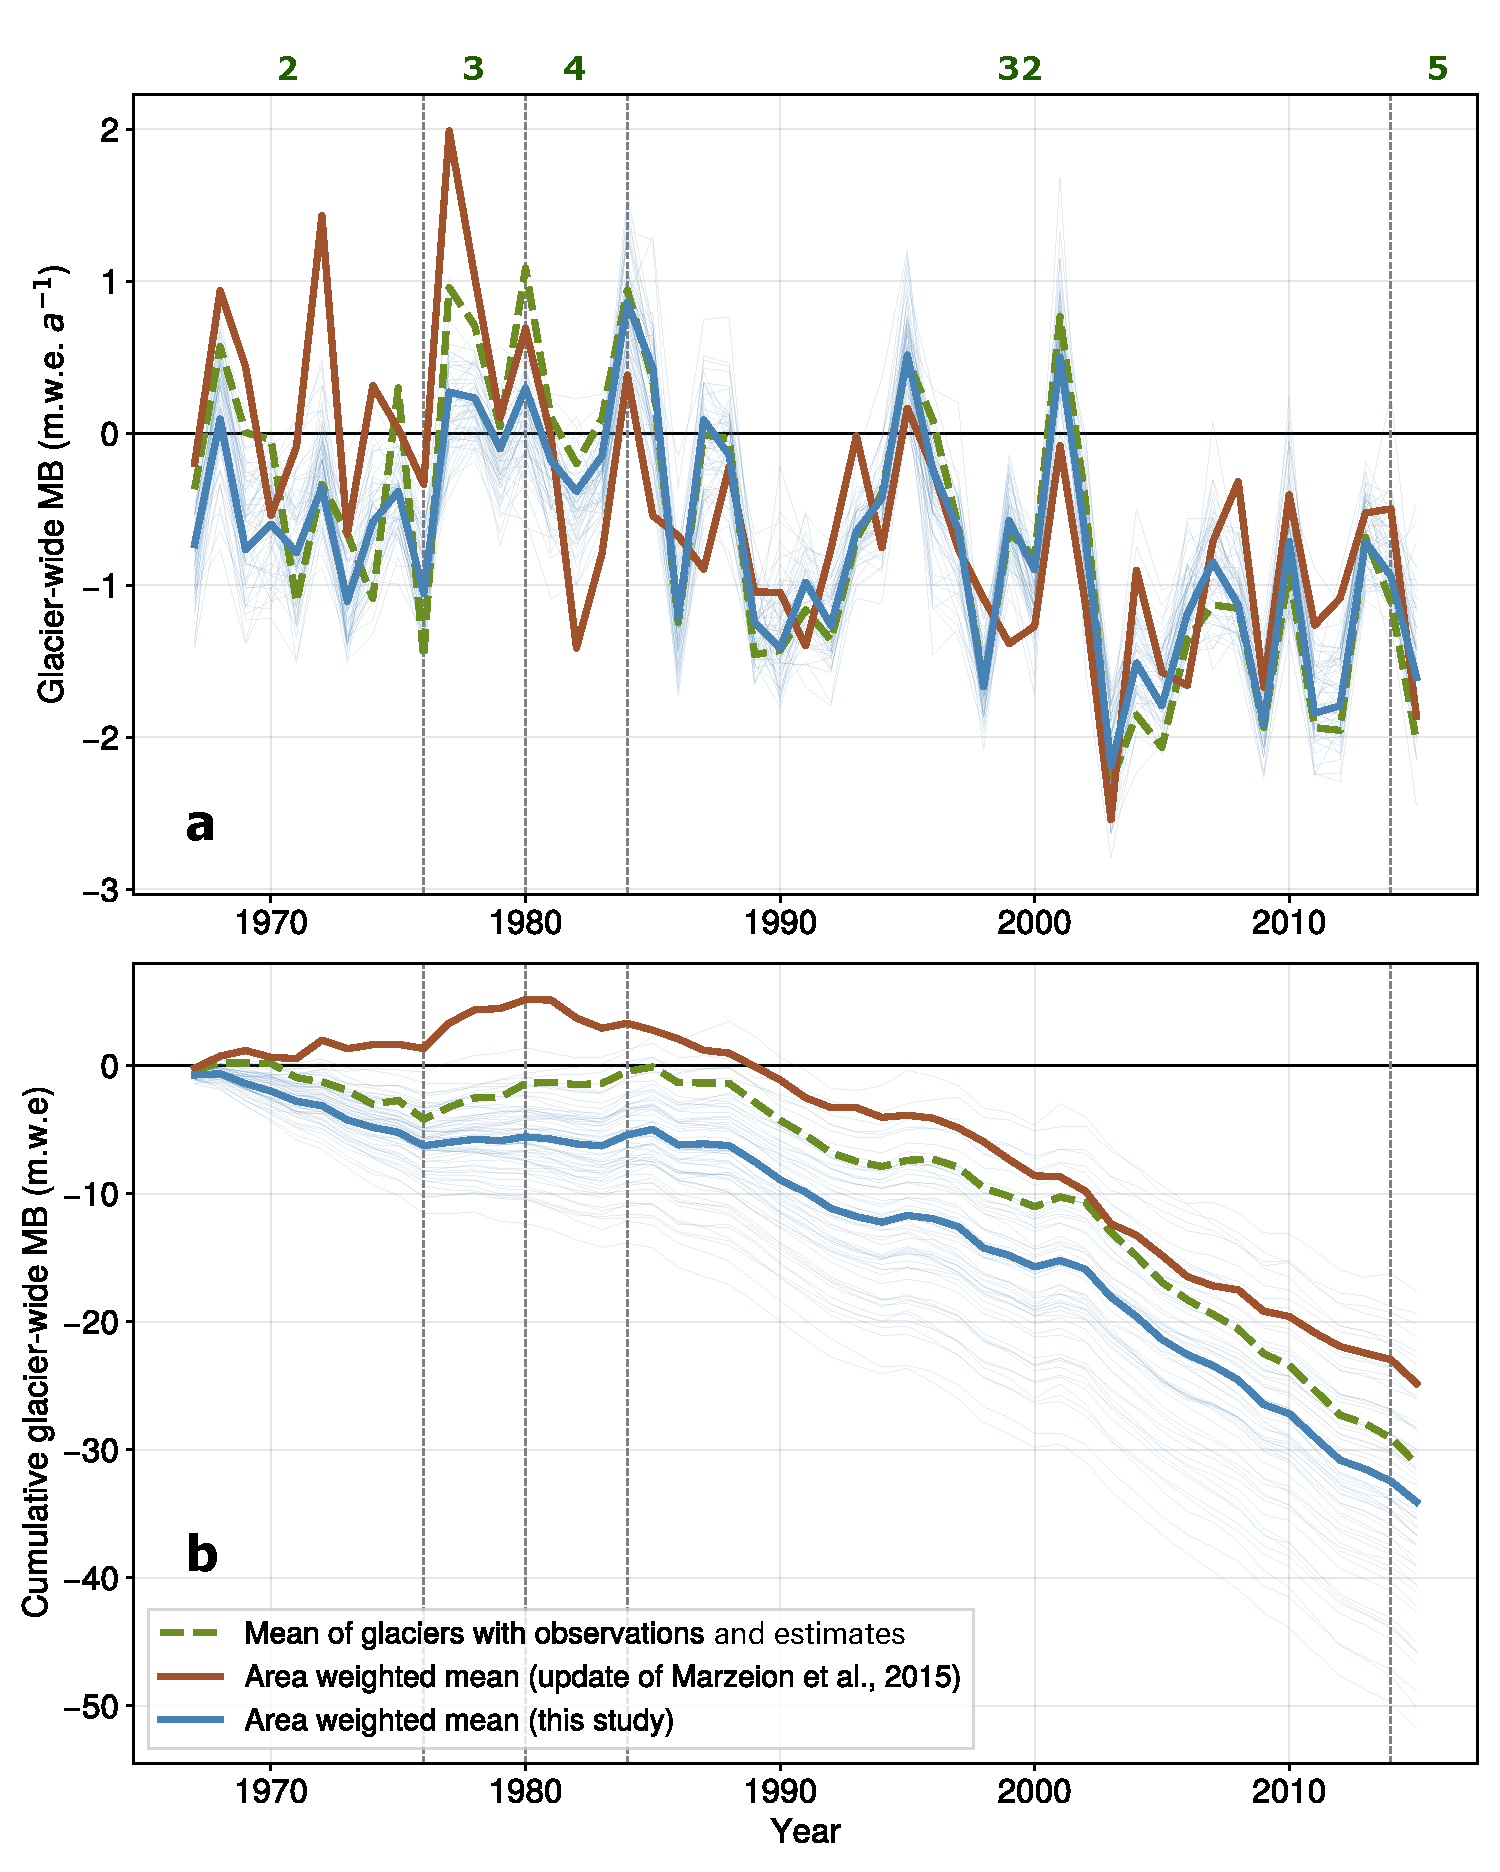
\includegraphics[width=10cm]{Figures/past/Figure_6.pdf}
\captionsetup{justification=centering}
\caption{Comparison of (a) annual and (b) cumulative glacier-wide MB simulations in the French Alps between this study, reconstructions from an update from Marzeion et al. (2015) and the mean of all observations and remote sensing estimates available in the French Alps. Green numbers indicate the number of glaciers with MB observations and remote sensing estimates for each period and thin light blue lines indicate the area-weighted mean of each of the cross-validation ensemble members.}
\label{past:fig6}
\end{figure}

In the following, we argue that similarities between observations, remote sensing estimates and the reconstructed glacier-wide MB values for the 1984-2015 period in this study (Fig. \ref{past:fig6}) are not due to overfitting. First, for the vast majority of the 661 French glaciers, the reconstructions are based on an ensemble of cross-validated models, which intrinsically limits overfitting (Sect. \ref{past:methods}).  Second, we analysed the deviation to the climatological mass-balance signal of the MB for each cluster of glacier-sizes. This analysis is presented in Sect. \ref{past:supp:overfitting} of the supplementary material. It reveals that the similarities between the training data and the reconstructed glacier-wide MB values for the 1984-2015 period in Fig. \ref{past:fig6} originate from big glaciers, that dominate both in the area-weighted reconstructions and in the training data (Fig. \ref{past:figS3} and \ref{past:figS4}). However, for the other glacier-size classes, our reconstruction shows different patterns from the data in the training data, which suggests that the model is not overfitting (Fig. \ref{past:figS3}). 

\section{Conclusions} \label{past:conclusions}

We presented a dataset of annual glacier-wide MB of all the glaciers in the French Alps (44° - 46°13’N, 5.08° - 7.67°E) for the 1967-2015 period \citep{bolibar_deep_2020}. This dataset has been reconstructed using deep learning (i.e. an artificial neural network), based on direct and remote sensing annual glacier-wide MB observations and estimates, climate reanalysis and topographical data from multitemporal glacier inventories. The deep learning model is capable of reconstructing glacier-wide MB time series for unobserved glaciers in the same region based on patterns and structures learnt by the artificial neural network from the training data and their relationships with predictors. An extensive cross-validation was implemented to understand the characteristics of the MB signal in the region and to assess the method’s validity and uncertainty. The average accuracy (RMSE) of the dataset is estimated at 0.55 m.w.e. a$^{-1}$ with an explained variance ($r^{2}$) of 75\%. Reconstructions show a mean area-weighted glacier-wide MB of -0.69±0.21 (1 $\sigma$) m.w.e. a$^{-1}$ for the 1967-2015 period. Important differences are found among different massifs, with the Mont-Blanc (-0.68 m.w.e. a$^{-1}$), Oisans (-0.75 m.w.e. a$^{-1}$ both) presenting the lowest mass losses and the Chablais (-0.93 m.w.e. a$^{-1}$), Champsaur (-0.86 m.w.e. a$^{-1}$) and Haute-Maurienne and Ubaye (-0.84 m.w.e. a$^{-1}$ both) showing the highest losses. In order to put these results into perspective, this reconstruction was compared to all available glacier-wide MB observations and remote sensing estimates in the French Alps as well as the physical/empirical reconstructions from another study \citep[update from][]{marzeion_brief_2015}. Interesting differences were found between the two methods, highlighting the different sensitivities and responses of different approaches to climate shifts that occurred during the study period. These differences are particularly relevant in the 1970s and 1980s, previous to a winter precipitation and summer temperature shift that occurred in the French Alps in the years 1976 and 1982, respectively. Moreover, after the famous 2003 European heatwave, glaciers experienced an acceleration in mass loss which is well captured by our reconstruction. This open glacier-wide MB dataset can be useful for hydrological or ecological studies in need of net glacier mass contributions of glacierized catchments in the French Alps. The publication of such open datasets is essential to future community-based data-driven scientific studies.

\section{Supplementary material}

\begin{figure}[h]
\centering
\includegraphics[width=12cm]{Figures/past/Figure_S1.pdf}
\captionsetup{justification=centering}
\caption{Comparison between glaciological observations from the GLACIOCLIM observatory, cross-validated MB reconstructions from this study (ANN CV) and fitted MB reconstructions (ANN). The cross-validated models are shown to display the out-of-sample performance. The fitted reconstructions display the actual reconstructions from the dataset, with models especially fitted for glaciers with data.}
\label{past:figS1}
\end{figure}

%\copyrightstatement{TEXT}

\subsection{Comparison with independent geodetic mass balance data} \label{past:supp:comparison}

All available annual glacier-wide MB data in the French Alps have been used to train the MB ANN of the present study. However, some multi-annual geodetic mass balance (MB) datasets exist that can provide a means to validate the reconstruction's bias for specific glaciers during multi-annual time intervals. This type of analysis is more limited than the cross-validation done to annual glacier-wide MB values in \cite{bolibar_deep_2020-1}, as it only gives information about the bias of a sub-period of the reconstructions instead of the accuracy found via cross-validation. Our MB reconstructions are compared against ASTER geodetic MB from \citet{davaze_region-wide_2020} for the 2000-2015 and 2003-2012 periods (Fig. \ref{past:fig2} and \ref{past:figS2}) and against Pléiades geodetic MB from \citet{berthier_glacier_2014} for the 2003-2012 period (Fig. \ref{past:figS2}).

For certain glaciers, the ASTER and Pléiades geodetic MB give a less negative MB than the glaciological SMB used to train the deep learning SMB model. This fact might explain the slightly more negative trend of our reconstructions seen for the 2000-2015 and 2003-2012 periods, which experienced very negative MB after the well known summer 2003 heatwave. This is quite surprising, since both the GLACIOCLIM glaciological MB measurements and the annual glacier-wide MB data from Rabatel et al. (2016) have been calibrated with geodetic MB from photogrammetric DEMs, which have a very high spatial resolution. For some regions (i.e. Grandes Rousses), the independent geodetic MB are well within the uncertainty range of our model. However, large and steep glaciers in the Mont-Blanc massif and some other regions, such as Bossons, Talèfre and Tour display important differences. These glaciers have very large and high altitude accumulation areas, not seen in almost any glacier in our training dataset. On the other hand, several small glaciers present very important differences, with ASTER-derived MB being much less negative than our reconstructions. Data for small glaciers carry very large uncertainties, often of the same order of magnitude as the observations themselves. On top of that, flat or dome-type glaciers with large white areas with high reflectance present an important amount of noise, further increasing the associated uncertainty. This means that is quite hard to jump to conclusions from a direct comparison between these glaciers and our reconstructions. The differences and influence of geodetic MB on the calibration of MB series should be properly studied, as they are often not taken into account as an additional uncertainty source. This topic goes beyond the scope of this study, but glacier modelling studies could benefit from integrating this in the list of uncertainties. 

\begin{figure}[t]
\centering
\includegraphics[width=12cm]{Figures/past/Figure_S2.pdf}
\captionsetup{justification=centering}
\caption{Comparison between glaciological observations from the GLACIOCLIM observatory (GC), ASTER geodetic mass balances from Davaze et al. (2020) (D20), the deep learning reconstructions from the present study (B20) and Pléiades geodetic mass balances from Berthier et al. (2014) (B14).}
\label{past:figS2}
\end{figure}

\subsection{Model differences between the updated version of Marzeion et al. (2015) and this study} \label{past:supp:diff}

In order to contrast the results from Sect. \ref{past:overview:comparison}, three important different aspects between our approach and the one of $M_{15U}$ need to be highlighted: 

\begin{enumerate}
\item $M_{15U}$’s model works with simplified physics, with a temperature-index model calibrated on observations; in this study we used a fully statistical approach based on deep learning, where physics-based considerations only appear in the predictor selection.
\item $M_{15U}$ calibrated their model with global MB observations, including 38 glaciers in the European Alps, most of them located in Switzerland for the 1901-2013 period; in this study we used observations of 32 glaciers, all located in the French Alps for the 1967-2015 period.
\item $M_{15U}$ forced their updated model with CRU 6.0 \citep[update of][]{harris_updated_2014}, with 0.5° latitude/longitude grid cells, which has a significantly lower spatial resolution and suitability to mountain areas than the SAFRAN reanalysis \citep{durand_reanalysis_2009} used in this study, in which altitude bands and aspects are considered for each massif, and meteorological observations from high-altitude stations are assimilated.
\end{enumerate}

The cross-validations of both studies determined a performance with an average RMSE of 0.66 m.w.e. $a^{-1}$ and an $r^{2}$ of 0.43 for $M_{15U}$ for the European Alps, and an average RMSE of 0.49 m.w.e. $a^{-1}$ and an $r^{2}$ of 0.79 for this study. However, due to the highly different methodologies and forcings of the two models, a direct comparison is not possible, so the following analysis is focused on the overall trends and sensitivities in the reconstructions and their potential sources. 

\subsection{Influence of area in glacier-wide MB signal and proof on non overfitting} \label{past:supp:overfitting}

Due to similarities between the averaged reconstructed glacier-wide MB and the observations during the 1984-2015 period, we decided to include an analysis to isolate the topographical influence in the glacier-wide MB signal, in order to verify that the model is not overfitting. Since the climate signal is the main common driver of annual variability of glacier-wide MB in the region, one needs to find a way to isolate the topographical signal. In Fig. \ref{past:figS3}, the median reconstructed annual glacier-wide MB of the 661 glaciers in the French Alps (i.e. the annual variability, hence a proxy of the climate signal) is subtracted to the mean annual values of the observations and of 4 subsets of glaciers divided by area classes. Therefore, one can observe the residual influence of glacier area on the glacier-wide MB signal. The influence of area on glaciers with observations is quite similar to glaciers with areas greater than 2 $km^{2}$, which is reasonable since glaciers with observations have an average of 4 $km^{2}$ (range: 0.3-31.8 $km^{2}$ in 2003). Moreover, one can see that even for a relatively short period of 30 years, the differences between the reconstructions for very small glaciers (< 0.5 $km^{2}$) and observations are quite important, accounting for an average cumulative loss of more than 5 m.w.e. As stated in Sect. \ref{past:methods}, this does not necessarily mean that the model has fully captured the topographical influence in the glacier-wide MB signal in the region, but it does prove that the model is not overfitting since it exhibits consistent variations in MB when the topographical predictors move away from the training data. Moreover, this is coherent with the importance attributed to topographical predictors \citep{bolibar_deep_2020-1}. 

The same analysis has been performed with the reconstructions from the updated version of Marzeion et al. (2015) (Fig. \ref{past:figS4}). The gradient with respect to glacier surface area appears to be similar, except for the behaviour of glaciers after 2007. Small and middle sized glaciers (0.1 - 2 $km^{2}$) switch to a positive influence, as opposite to large glaciers (> 2 $km^{2}$), which transition to a negative influence. Conversely, our results show a more continuous trend, without a change of behaviour in the last years of the analysed period. 

\newpage
%\break
\subsection{Supplementary figures}

\begin{figure}[h]
\centering
\includegraphics[width=16cm]{Figures/past/Figure_S3.pdf}
\captionsetup{justification=centering}
\caption{Influence of glacier area on the glacier-wide MB signal. The reconstructed median annual glacier-wide MB of the 661 glaciers in the French Alps can be seen as a proxy of the climate signal in the region. It is subtracted to the mean annual glacier-wide MB of the glaciers with observations and to four different subsets of reconstructions divided into glacier area size, showing only the annual differences based on glacier area classes. The dotted line depicts the subtracted signal (non cumulative) in order to give some context.}
\label{past:figS3}
\end{figure}

\begin{figure}[h]
\centering
\includegraphics[width=14cm]{Figures/past/Figure_S4.pdf}
\captionsetup{justification=centering}
\caption{Same as S3 but comparing this study to the updated version of Marzeion et al. (2015). In the legend, “B” stands for Bolibar et al. (this study) and “M” for the update of Marzeion et al. (2015). Both models show a relatively similar gradient effect with respect to glacier area, with differences in the amplitude of the effects. The main differences appear from 2007, where small and middle sized glaciers (0.1 - 2 $km^{2}$) from the update of Marzeion et al. (2015) switch to a positive influence, as opposite to large glaciers (> 2 $km^{2}$), which transition to a negative influence. The reconstructed MB dotted lines are not cumulative and they are depicted in order to give some context of the subtracted climate signal.}
\label{past:figS4}
\end{figure}


\begin{figure}[t]
\centering
\includegraphics[width=9cm]{Figures/past/Figure_S5.png}
\captionsetup{justification=centering}
\caption{Cross-validation for annual glacier-wide MB values outside the main 1984-2014 training period. The black line indicates the one-to-one reference. Simulations have been done from 1959, the earliest date with observations to validate against the maximum number of values. This serves to confirm that the model is capable of reproducing glacier-wide MB outside the main observed period.}
\label{past:figS5}
\end{figure}


\begin{figure}[t]
\centering
\includegraphics[width=16cm]{Figures/past/Figure_S6.pdf}
\captionsetup{justification=centering}
\caption{Average annual glacier-wide MB for each glacier over the entire study period with respect to (a) glacier surface area, (b) the lowermost 20\% altitudinal range slope and (c) mean glacier altitude. p indicates the p-value and r the correlation between the topographical variables and the average glacier-wide MB.}
\label{past:figS6}
\end{figure}


\begin{figure}[t]
\centering
\includegraphics[width=12cm]{Figures/past/Figure_S7.pdf}
\captionsetup{justification=centering}
\caption{Comparison of area-weighted decadal glacier-wide MB simulations in the French Alps between this study and an update from Marzeion et al. (2015).}
\label{past:figS7}
\end{figure}


\begin{figure}[t] 
\centering
\includegraphics[width=16cm]{Figures/past/Figure_S8.pdf}
\captionsetup{justification=centering}
\caption{Average annual glacier-wide MB per glacier area classes}
\label{past:figS8}
\end{figure}


\begin{figure}[t]
\centering
\includegraphics[width=16cm]{Figures/past/Figure_S9.pdf}
%\captionsetup{justification=centering}
\caption{Average annual glacier-wide MB for classes of glacier slope of the lowermost 20\% altitudinal range (i.e. a proxy of the glacier’s tongue slope)}
\label{past:figS9}
\end{figure}



\chapter{The 21$^{st}$ century deglaciation of the French Alps: unraveling climate-glacier interactions with deep learning}
\label{chap:future}

\begin{flushright}
{\small \textit{All models are wrong, but some are useful.}\\
George Box}
\end{flushright}

\section*{Preface}




\part{Glacierized mountain catchments}

\chapter{Glacio-hydrological modelling of glacierized mountain catchments}
\label{chap:discussion}

\begin{flushright}
\begin{small}
\textit{Water is the driver of nature.}\\
Leonardo da Vinci
\end{small}
\end{flushright}

\section*{Preface}

This second part of the manuscript is driven by the BERGER project, which combines the glacio-hydrological modelling efforts presented here with an ecological study on the impacts of glacier retreat on aquatic communities and their adaptation in the French Alps. An unexpected shift in the initial objectives of this PhD project resulted in a lengthy investigation of machine learning methods applied to glacier evolution modelling, which impacted the initial plans for glacio-hydrological modelling. Efforts for this part of the PhD work have been focused on the technical implementation and validation of a novel glacier component for a hydrological model. With this implementation, we are providing the technical means for an application on glacio-hydrological studies at a regional scale in the French Alps. This work has been done with the help of Sven Kralisch from the University of Jena (Germany). His expertise on the hydrological model used in this study has greatly helped to accelerate the development of the updated glacier module in the last months of this project.

\section{Introduction}

Glaciers supply water that supports ecosystems and human communities both nearby and far away from glaciers \citep{ipcc_climate_2018}. The strong climatic diversity of glacierized alpine catchments enables the storage of precipitation in the form of snow and ice at high altitudes. In the European Alps, this water storage is progressively released throughout the year during the warmest months, providing a base-flow that cannot be encountered in non-glacierized catchments. At the beginning of the melt season, snow provides important water resources downstream. Once most of the snow has melted, leaving bare glacier ice exposed, glaciers continue providing freshwater resources, ensuring an uninterrupted runoff throughout the melt season \citep{huss_toward_2017}. In one of the few existing glacio-hydrological studies in the French Alps, \citet{lafaysse_influence_2011} estimated that melt water from glaciers contributed to 20\% of the August discharge of the Durance at Serre Ponçon catchment (3500 km$^{2}$). According to \citet{huss_present_2011} in a study using a simple routing of glacier discharge, glaciers contributed to 25\% of the summer low flow of the Rhone river (about 100000 km$^{2}$ in catchment size), with an even enhanced contribution during the 2003 drought. This role of glaciers as late summer buffers is currently being challenged by anthropogenic climate change. Glacier retreat in the European Alps is progressively transforming the hydrological regime of high-mountain catchments, with potential environmental and social impacts \citep{zekollari_modelling_2019}. In the French Alps, the local population have a strong dependency on water resources, using them for agriculture, hydropower generation and domestic use. The regional socioeconomic model of many alpine valleys is built around mountain tourism, with a strong dependency on the cryosphere, both as a tourism attraction \citep{schut_sport_2013, spandre_winter_2019} and as an electricity generation source \citep{schaefli_role_2019}. Moreover, late summer runoff from glaciers provides reliable water resources for domestic use, industries and agriculture. The decrease in glacier freshwater contributions has ecological impacts as well, affecting biodiversity in glacier-fed rivers \citep{cauvy-fraunie_global_2019} and in humid areas that no longer receive runoff during the warmest period of the year \citep{carlson_monitoring_2020}. Glaciers provide cold water resources that help regulate the temperature, flow regimes, sediment concentration and nutrient supply of mountain streams \citep{huss_toward_2017}. These cold waters are essential to some specialized species, whose survival will be challenged by glacier retreat \citep{lencioni_glacial_2018, cauvy-fraunie_global_2019}. Alternatively, these changing streams can be quickly colonized by aquatic communities adapted to higher water temperatures, increasing competition between species  \citep{robinson_ecosystem_2014}. Anticipating these future hydrological changes is of paramount importance in order to correctly adapt and manage future water social and environmental needs. 

Hydrological models can provide answers to these questions, predicting the hydrological evolution under different future climate scenarios. In France, multiple hydrological models are being developed and used for research and operational purposes. At one end of the spectrum of model complexity, the lumped GR rainfall-runoff models, with the CemaNeige snow component \citep{coron_suite_2017}, use a simplified modelling approach with catchment-scale representations of the transformation of precipitation into discharge. They rely on the calibration of 1 to 6 parameters (depending on the model variant and time-step), and do not include a glacier component. This limits their usability in high-altitude, upstream catchments where observational data is scarce and glaciers may play an important role.  At the other end of the complexity spectrum, the physics-based SIM (SAFRAN-ISBA-MODCOU) model combines a meteorological analysis system (SAFRAN), with a land surface model (ISBA) and a hydrogeological model (MODCOU) developed by the Mines de Paris \citep{habets_safran-isba-modcou_2008}. For research purposes, it has been adapted to alpine areas by incorporating elevation bands, aspect classes, and  glacier melt and retention of underground water \citep{lafaysse_influence_2011}. However its adaptation and deployment over the entire French alpine region, including glacierized areas, is highly demanding \citep[e.g.][]{lecourt_physically-based_2018} and has not been considered yet. For more operational applications, the reservoir-based MORDOR model \citep{paquet_evolution_2004}, developed by Électricité de France (EDF), has a more intermediate complexity. It is actively  used to forecast runoff in mountain catchments in France and to anticipate changes in hydropower production, both for short and long term periods. However this model is not open to applications outside the scope of EDF operational and research objectives. Finally, The GSM-Socont model \citep{schaefli_conceptual_2005}, a Swiss semi-distributed glacio-hydrological model, has been recently applied to perform projections of the Arve watershed in the Mont-Blanc massif through the 21${st}$ century \citep{laurent_impact_2020}. Out of all these models, only the GSM-Socont model includes a dynamic representation of glaciers, and \citet{laurent_impact_2020} is the first study of this kind in a French glacierized catchment. The vast majority of hydrological models deployed in France have none, or a very simplified representation of glaciers, including them as static ice reservoirs. Some models do have such glacier modules, but they are not activated due to a lack of data to calibrate and validate them. Such a representation is problematic in the current context of glacier retreat, neglecting future changes in hydrological regimes driven by glaciers. 

This static representation of glaciers is also found in the J2K hydrological model \citep{krause_quantifying_2002}, developed at the University of Jena (Germany). J2K is a semi-distributed open-source model, based Hydrological Response Units (HRUs), homogeneous spatial units in terms of hydrological processes. It allows the representation of multiple physical processes, land use covers, pedology, geology and topography. Moreover, the representation of multiple anthropogenic water uses, such as agriculture irrigation or reservoir management dams can be taken into account into the model. J2K is being used by a large community of hydrologists, both in France and internationally, for a wide variety of geographical configurations \citep{krause_quantifying_2002, nepal_understanding_2014, braud_j2000-rhone_2017}. J2K has already been applied to glacierized catchments in the Himalayas \citep{nepal_understanding_2014}, but simulations have only been performed for past periods, keeping the glacier surface area constant in time. In this chapter, I present an updated glacier module for J2K, including a dynamic representation of glaciers. We introduce and validate this new implementation in a partially-glacierized alpine catchment in the French Alps: the Arvan catchment in the Grandes Rousses massif. By introducing glacier evolution in a hydrological model, we aim at improving hydrological simulations and discharge projections out of glacierized catchments, in order to assess the impacts of these changes on aquatic communities living in glacier-fed streams. 

\section{Methods}

\subsection{Study area}

The Arvan catchment (58.8 km$^{2}$, Fig. \ref{hydro:figA1}) is a partially glacierized alpine catchment, located in the Grandes Rousses massif, between 1368 and 3373 m a.s.l. It includes the Saint-Sorlin Glacier (2.069 km$^{2}$ in 2015, 3.5\% of glacial coverage at catchment scale), being the glacier with the second longest mass balance observation series in France (1957-present). Two villages are located within the catchment: Saint-Sorlin-d'Arves and Saint-Jean-d'Arves, with the latter including water flow measurements for the 2000-2016 period. This study site has been chosen due to its wealth of glaciological, meteorological and hydro-biological data, providing an adequate testbed to validate the modelling approach within the context of the BERGER project.

\subsection{Data}

This work has been implemented in a version of J2K dedicated to the Rhône river catchment, situated in France and Switzerland. Therefore, most of the datasets used (except the climate data) have a full coverage of this geographical region.

\subsubsection{Climate}

The J2K hydrological model is forced with climate data coming from SPAZM \citep{gottardi_statistical_2012}. SPAZM is a statistical method to interpolate meteorological data, particularly precipitation, in mountain areas. This interpolation has been applied on French mountainous regions, based on an observational network, taking into account the local orography and the main atmospheric patterns bringing precipitation. With a resolution of 1 km$^{2}$, this dataset is well adapted to representing the complex meteorological conditions of a glacierized alpine catchment. Temperature and precipitation are available from the year 1953 until the end of the year 2012, which suit the needs of J2K.

\subsubsection{Land cover}

Land cover use is determined by the Corine Land Cover 2006 (CLC2006) European database. It has a minimum vectorial detail of 25 ha and it takes into account a maximum of 44 different land cover uses. Land use data is used to determine certain variables in different hydrological processes, such as the surface albedo or the leaf area index. 

\subsubsection{Pedology}

Pedology information is used to estimate the size of the superficial soil reservoirs in the model. The following databases have been used to describe pedology: The Soil European Database, providing soil thickness data; and the ECOCLIMAP database, with a 1 km resolution, describing soil texture. The representation of these superficial soil reservoirs is based on \citet{sauquet_risk_2014}, adapted for mountain territories. 

\subsubsection{Geology}

Geology data is taken from the Bureau des Recherches Géologiques et Minières (BRGM) dataset, grouped in eight different classes, five of which are dominant in the French Alps: fluvioglacial deposits, shale and metamorphic rocks, detrital rocks, limestone and marls. In J2K, geology is used to determine the size and time to empty the deep ground reservoirs. 

\subsubsection{Hydrology}

Hydrological observations at the Saint-Jean-d'Arves station (Fig. \ref{hydro:figA1}), are available with a daily frequency for the 2000-2016 period. This data is compiled as part of DREAL Rhône-Alpes's database of hydrological observations \citep{brigode_summary_2020}. This station measured an average interannual flow of 1.8 m$^{3}$/s, with 10\% of temporal gaps for this period and a low reliability of winter measuremets due to snow and ice (Fig. \ref{hydro:figA1}).

\subsubsection{Glaciology}

Several different datasets are available for the Saint-Sorlin Glacier. Seasonal (winter and summer) point MB data from the GLACIOCLIM French national observatory are available at 30 different points since 1995. Glacier-wide MB observations, performed every year in September, cover the 1957-2019 period. Seasonal glacier-wide MB data were computed specifically for the 2000-2010 period \citep{davaze_monitoring_2018}. Glacierized surface areas for this glacier proceed from the results of model simulations using the ALPGM model, introduced in Chapter 2. 

\subsection{The J2K hydrological model}

J2K is an open-source hydrological model coded in Java. It is structured in Hydrological Response Units (HRUs), irregular spatial divisions representing homogeneous conditions from a hydrological point of view. HRUs are determined by a combination of different spatial data, such as the surface slope, altitudes from a DEM, vegetation cover, geology and the distribution of sub-catchments. For the J2K model version used in our study, HRUs are determined by taking into account the sub-catchments with control gauging stations from the hydrological network of observations. These control points are used for model calibration and validation, enabling a comparison of model simulations with observations. The automatic generation of HRUs is performed with a special tool named HRU-delin, providing the modelling structure for any given catchment with the required data. The physical characteristic of each HRU are stored in specific files, which are used by the model to simulate different hydrological processes. 

Simulations are performed separately for each HRU (Fig. \ref{hydro:fig1}). Total precipitation can be partially intercepted by vegetation, whose remaining fraction that reaches the ground will be further divided into infiltrated and surface runoff (RD1) fractions. Infiltrated water will first fill a Large Pore Space (LPS) reservoir, which can then be transferred towards a Medium Pore Space (MPS) reservoir (Fig. \ref{hydro:fig1}). Evapotranspiration is mainly retrieved from water intercepted by vegetation and water available in the MPS reservoir. It is computed on vegetation following the Penman-Monteith reference potential evapotranspiration \citep{howell_penman-monteith_2004}. J2K allows ground water to form subsurface runoff (RD2) if the surface slope is steep enough or the substrate has low infiltration. The remaining fraction is assumed to percolate towards a deep reservoir (RG1). The simulated total water flow within an HRU is equivalent to the sum of the runoff, the subsurface flow and a slow flow from the deep reservoir. Water flow is routed among HRUs via streams if the HRU is located on a valley bed. Conversely, HRUs not containing a water stream route their water flow towards neighbouring HRUs using a simplified kinematic wave method \citep{chen_surface_1970}. Every type of water storage (e.g. RD1, RD2) from each HRU is routed separately until reaching the catchment's outlet. 

\begin{figure}[h]
\centering
\includegraphics[width=10cm]{Figures/hydro/Figure_1.png}
\caption{Workflow of the J2K hydrological model. \textit{Slightly edited from the J2K documentation.}} 
\label{hydro:fig1}
\end{figure}

J2K establishes a simulation workflow using temporal (HRU-Loop) and spatial (Time-Loop) contexts, which iterate and perform simulations for each HRU and day of a given catchment and time period. These contexts are implemented in the Jena Adaptable Modelling System (JAMS) platform, in which J2K is integrated. The simulation of specific hydrological processes are performed in components, being separate entities taking a given set of input parameters, processing them and returning multiple output parameters. 

\subsection{An updated glacier module for J2K}

In J2K, the generation of HRUs for a certain catchment can only be done prior to model simulations. The extent and content of HRUs is static in time, preventing the model from making them evolve throughout a simulation. This specificity of J2K makes it difficult for the model to include a dynamic representation of glaciers, explaining why all simulations for glacierized catchments have so far been performed with static glacierized areas \citep{gao_test_2012, nepal_understanding_2014}. In order to overcome this limitation, we have developed an approach allowing the introduction of glacier evolution through time, based on prescribed glacier surface areas fed to the model at a regular timestep (e.g. daily in this study). 

A Python package named \textit{Glaciers-to-J2K} has been created, which automatically computes the glacierized fraction of each HRU based on polygons with the extension and surface type of each HRU and annual glacier boundaries. Glacier boundaries can proceed from any glacier model providing annual gridded glacier extents. \textit{Glaciers-to-J2K} computes the glacierized and non-glacierized fraction of each HRU by overlapping HRU outlines with annual glacier extents. Then, these fractions are interpolated with a daily timestep throughout a given ablation season, with a default period between October 1${st}$ to March 31${st}$. This enables a daily representation of glacier area evolution, necessary for hydrological simulations with J2K. These time series are stored in a \textit{.dat} file.

Several components of J2K have been adapted in order to take into account these changes in glacier surface area. 

\subsubsection{Glacier dynamics}

Two new components named \textit{GlacierFractionReader} and \textit{GlacierFractionAssigner} have been added, responsible for reading the daily glacierized fractions for each HRU and assigning them to the right HRU during the temporal (Time-Loop) and spatial (HRU-Loop) iterations. 

\subsubsection{Glacier mass balance and runoff}

[Eric: partie compliquée à suivre: on ne sait pas où se positionne le module dans le schéma 5.1; les variables d'état ne sont pas précisées, les paramètres fixes ou à caler (par HRU ou régionalement) ne le sont pas non plus, les unités non plus quand les équations sont fournies; parfois le temps t est indiqué (suggestion utiliser d pour day car il y a une variable tsnow); newSnowDens = snowDens(t) par comparaison à snowDens(t-1); peut être organiser différemment : description du glacier (variables et paramètres), processus de formation, destockage potentiel, croisement des deux (estimation des flux sortants) et mise à jour des états, donc réorganiser ton texte et ne pas hésiter à changer des noms de variables du code par des noms plus explicites] An already existing glacier module from the J2K model version used in the Himalayas has been updated, creating a new module named \textit{GlacierModuleAlps}. If the glacierized fraction of a given HRU is different than zero, a glacier is detected and the simulation of glacier runoff is triggered. First of all, the snowpack on the glacier is processed with a dedicated snow component, determining the characteristics of snow on the glacier. It simulates accumulation and compaction of the snow pack caused by snow melt or rain. The thermal characteristics under the snow pack are also taken into account with the cold content (CC) of snow (Eq. \ref{hydro:eq:1}).

\begin{equation} \label{hydro:eq:1}
 ColdContent = coldContFact \cdot T
 \end{equation} 
 
where $coldContFact$ is a calibration parameter and T the air temperature at a given HRU. This enables the accumulation of negative temperatures, which are decreased only by positive temperatures, resulting in a potential melting rate. Melting is triggered once the CC [Eric: j'ai beau cherché CC n'est pas utilisé plus loin; pas clair à quoi sert la variable; seuil pour déclencher la fonte ? pourquoi ne pas utiliser que la température ?] has reached zero. Snow occurs when precipitation falls with air temperatures lower than 0ºC. The density of new snow is determined by air temperature follow equation \ref{hydro:eq:3}.

\begin{equation} \label{hydro:eq:2}
 newSnowDens = 0.13 + 0.0135 \cdot T_{acc} + 0.000045 \cdot T_{acc}^{2}
\end{equation} 
 
where $T_{acc}$, which shares the same formulation as the melting temperature ($T_{melt}$), is defined by equation \ref{hydro:eq:3}.

\begin{equation} \label{hydro:eq:3}
 T_{acc} = T_{melt} = \frac{T_{min} + T_{avg}}{2}
\end{equation} 

[Eric: j'ai utilisé l'équation 5.2 et j'obtiens  -0.062375 = 0.13+0.0135*-15+0.000045*15*15 avec Tacc=-15°C] If air temperature is lower than -15ºC the density of snow is assumed to be 0.02875 g/cm$^{3}$. At this point, the change in snow depth ($\Delta SH$) from snowfall is determined by equation \ref{hydro:eq:4}.

\begin{equation} \label{hydro:eq:4}
 \Delta SH = \frac{snow}{newSnowDens}
\end{equation} 

Then, the snow water equivalent (SWE) of the previous day ($SWE_{dry}$) is increased with new snow, following equation \ref{hydro:eq:5}.

\begin{equation} \label{hydro:eq:5}
 SWE_{dry,t} = SWE_{dry,t-1} + snow
\end{equation} 

[Eric: SWEdryt ou SWEtott?] If $T_{melt}$ exceeds a certain threshold value (normally 0ºC) the snow pack transitions from accumulation phase to metamorphosis. The amount of energy available for melt is computed in three different ways: (1) the sensible heat from air temperature ($t_{snow}$), (2) the energy input from rain ($r_{factor}$), and (3) the energy input from soil heat flow ($g_{factor}$). The sum of these three components gives the potential snow melt rate ($M_{p}$), defined by equation \ref{hydro:eq:6}.

\begin{equation} \label{hydro:eq:6}
 M_{p} = (t_{snow} \cdot T_{melt} + r_{factor} \cdot rain \cdot T_{melt} + g_{factor}) \cdot \theta
\end{equation} 

where $\theta$ is a parameter [Eric: calibrated? fixed?] modifying the melt according to the slope and aspect of the HRU. At this point, $M_{p}$ is used to update the $ColdContent$ and the maximum change in the snow pack (Eq. \ref{hydro:eq:7}).

\begin{equation} \label{hydro:eq:7}
 \Delta SH = \frac{M_{p}}{dry_{density}}
\end{equation} 

where $dry_{density}$ is the snow dry density. If $\Delta SH$ is greater than the entire snow depth, it melts completely and the entire SWE contributes to runoff generation. If this is not the case, $SH$ is reduced accordingly, leading to an increase in the total snow density ($tot_{dens}$). Additionally to this change of density, changes in subsidence and density following the snow compaction scheme \citep{bertle_effect_1966} are taken into account. Water seeps into the snow pack, contributing to subsidence by recyrstallization of snow and by structural changes. This subsidence rate is computed using the snow-subsidence method, whose increase of accumulated water content in percentage is determined by equation \ref{hydro:eq:8}.

\begin{equation} \label{hydro:eq:8}
 P_{w} = \frac{SWE_{tot}}{SWE_{dry}}100
\end{equation} 

The greater the liquid water in input, the greater the snow pack subsidence will be. The percentage of snow depth change ($P_{H}$) is computed from the input of free water (Eq. \ref{hydro:eq:9}).

\begin{equation} \label{hydro:eq:9}
 P_{H} = 147.4 - 0.474 \cdot P_{w}
\end{equation} 

allowing the calculation of the new snow depth ($SH$).

\begin{equation} \label{hydro:eq:10}
SH = SH\frac{P_{H}}{100}
\end{equation} 

Finally, the dry snow density ($dry_{dens}$) and the total snow density ($tot_{dens}$) are recomputed taking into account this updated snow depth (Eqs. \ref{hydro:eq:11} and \ref{hydro:eq:12}). 

\begin{equation} \label{hydro:eq:11}
dry_{dens} = \frac{SWE_{dry}}{SD}
\end{equation} 

\begin{equation} \label{hydro:eq:12}
tot_{dens} = \frac{SWE_{tot}}{SD}
\end{equation} 

[Eric: SD? drydens = drydensity introduit plus haut?]The snow pack can store liquid water in its pores up to a certain critical density ($snow_{critDens}$). When a certain amount of liquid water is reached with respect to the total SWE (about 40-45\%), this storage is released \citep{bertle_effect_1966}. This process is taken into account in the model by computing a maximum water content in the snow pack ($SWE_{max}$), following equation \ref{hydro:eq:13}.

\begin{equation} \label{hydro:eq:13}
SWE_{max} = snow_{critDens}\cdot SD
\end{equation} 

The $snow_{critDens}$ needs to be provided by the user. Finally, the snow runoff ($Q_{snow}$) is determined by the water stored in the snow pack that exceeds this limit [Eric: dans l'équation introduire max[SWEtot-SWEmax;0](Eq.\ref{hydro:eq:14}).

\begin{equation} \label{hydro:eq:14}
Q_{snow} = SWE_{tot} - SWE_{max}
\end{equation} 

Through time (daily time steps in our case), the snow pack can keep this critical threshold density until being defrosted or new snowfall occurs. 

If no snow is present in a given glacierized HRU, ice melt can occur. This is computed using a temperature-index melt model \citep{hock_temperature_2003}, following equation \ref{hydro:eq:15}.

\begin{equation} \label{hydro:eq:15}
ice_{melt} = \frac{1}{n}t_{ice} + \alpha_{ice } \cdot Q_{radiation} \cdot(T_{melt} - T_{base})
\end{equation} 

where $n$ is the time stemp ($n$ = 1 for a daily model), $t_{ice}$ is a melt factor specific for ice, $\alpha_{ice}$ is a fixed ice melt coefficient based on albedo, $Q_{radiation}$ is the actual global net solar radiation at the surface and $T_{base}$ is a based temperature defined by the user to trigger melt (normally 0ºC). The previously existing glacier module implemented in the Himalayas also takes into account the effects of debris cover, which will not be described here since they have not been implemented in this work due to time constraints. 

Finally, snow melt and ice melt are further adapted depending on the slope and aspect of each HRU (Eqs. \ref{hydro:eq:16} and \ref{hydro:eq:17}).

\begin{equation} \label{hydro:eq:16}
Q_{snow} = (r_{t-1 }\cdot e^{(1/k_{snow})} \cdot Q_{snow} \cdot e^{(1/k_{snow})}) \cdot g_{fraction}
\end{equation} 

\begin{equation} \label{hydro:eq:17}
Q_{ice} = (r_{t-1} \cdot e^{(1/k_{ice})} \cdot Q_{ice} \cdot e^{(1/k_{snow})}) \cdot g_{fraction}
\end{equation} 

where $r_{t-1}$ is the outflow reservoir during the previous time step[Eric: which reservoirs?]; $k_{snow}$ and $k_{ice}$ are storage coefficients for the reservoirs, determined by the user; and $g_{fraction}$ is the glacierized fraction of the HRU, used to scale the runoff coming from glaciers. 

The resulting daily glacier MB for each HRU is calculated from the input precipitation and the output ice ($Q_{ice}$), snow ($Q_{snow}$) and rain ($Q_{rain}$) flows (Eq. \ref{hydro:eq:18}).

\begin{equation} \label{hydro:eq:18}
MB = (rain + snow - Q_{ice} - Q_{snow} - Q_{rain}) \cdot g_{fraction}
\end{equation} 

\subsubsection{Non-glacierized fraction}

Glacierized HRUs might contain a non-glacierized fraction as well. The runoff computed outside the glacier, within the previously existing workflow in J2K, is multiplied by the non-glacierized HRU fraction ($1 - g_{fraction}$). This enables an accurate separation between glacierized and non-glacierized runoff contributions for each HRU. 

\subsubsection{Mass balance calibration}

Therefore, this updated glacier module computes glacier mass balance with a daily timestep. In order to correctly calibrate glacier mass balance, three parameters can be tuned: a precipitation lapse rate specific for the glacier, a snow melt factor ($t_{snow}$) [Eric: better to keep the same name throughout the text cf. Eq. 5.6] and an ice melt factor ($t_{ice}$). Precipitation is known to be underestimated at high altitde (> 3000 m a.s.l.) in climate datasets in the French Alps, for both the SAFRAN and SPAZM datasets used in this PhD work \citep{vionnet_numerical_2016}. This means that increasing precipitation via a lapse rate factor is often needed in order to correctly reproduce accumulation rates on glaciers. 

This implemented approach can be easily escalated [Eric: upscaled? extended?] to glacierized catchments with multiple glaciers. Every HRU has an ID which can be matched to any Randolph Glacier Inventory (RGI) ID, allowing a specific calibration of mass balance models for each individual glacier. In catchments with small glaciers located close together, these might end up sharing an HRU. For these cases, the optimization of the melt model would have to be shared among all the glaciers present in that HRU. Alternatively, the size of the HRU separation can be reduced, improving the spatial representation of the catchment. Nonetheless, this has an important computational cost. We believe this updated modelling framework has enough flexibility to enable an accurate calibration of different melt factors and precipitation lapse rates in mountainous regions. 

\section{Results}

This updated glacier module for the J2K hydrological model has been implemented and validated in the Arvan partially glacierized catchment at Saint-Jean d'Arves in the French Alps (Fig. \ref{hydro:fig2}). In this catchment configuration, the Saint-Sorlin Glacier occupies four different HRUs, whose glacierized fraction and surface area has been computed for every year between 2003 and 2012 using glacier ice thickness data simulated with ALPGM \citep{bolibar_alpgm_2020}.[Eric: in the legend, Hyrological ==> gauging station; in blue extension of the glacier in 2003]

\begin{figure}[h]
\centering
\includegraphics[width=12cm]{Figures/hydro/Figure_2.pdf}
\caption{The Arvan catchment at Saint-Jean d'Arves, with its division into HRUs and their main land use. } 
\label{hydro:fig2}
\end{figure}

\subsection{Glacier evolution}

The evolution of glaciers in the updated glacier module of J2K is represented with prescribed annual glacier extents taken from an independent glacier evolution model. For this case study, ALPGM provided annual glacier ice thickness data from the year 2003, where initial glacier ice thickness data are available from \citet{farinotti_consensus_2019}. The 1985-2003 period was used as a spin-up period for the model, in order to correctly initialize the water reservoirs and snow pack. During the spin-up period, since no glacier ice thickness data is available, the extent of the glacier was kept the same as the year 2003. We consider this approximation to be acceptable, taking into account that this simulated period is only used as spin-up. The match between the initial glacier ice extent and the catchment HRUs was not perfect, with small parts of the glacier exceeding the HRUs extent (Fig. \ref{hydro:fig2}). The prescribed glacier surface areas by the ALPGM glacier model also carry uncertainties, particularly from the initial glacier ice thickness. Simulated glacier MB data for this period have a very small error (Fig. 3.7), and the parameterization used to update the glacier geometry was specifically calibrated for this glacier. [Eric: fig 5.3 not cited]These uncertainties resulted in the simulated glacier geometry only evolving in thickness but not extent between 2004 and 2006. This can be seen in the prescribed glacier surface area changes, which do not evolve until early 2006 (Fig. \ref{hydro:fig3}). As soon as the prescribed glacier surface area evolved, J2K captures a realistic glacier area evolution during the ablation season. The overall glacier surface area in J2K is correctly represented, despite the slight mismatches in glacier and HRU data. The Saint-Sorlin glacier displayed a total surface area of 2.79 km$^{2}$ in the year 2003 \citep{gardent_multitemporal_2014}, very close to the 2.66 km$^{2}$ obtained in J2K (Fig. \ref{hydro:fig3}). 

\begin{figure}[h]
\centering
\includegraphics[width=10cm]{Figures/hydro/Figure_3.pdf}
\caption{Daily evolution of the glacierized surface area of Saint-Sorlin Glacier in J2K. Glacier retreat during the ablation season is well captured in the model, following the prescribed interpolated area evolution. The glacier area is only updated from October 2003 onwards, after the first year with available glacier ice thickness data.} 
\label{hydro:fig4}
\end{figure}

\subsection{Glacier mass balance}

In order to calibrate the temperature-index model in J2K for the Saint-Sorlin Glacier [which equations?], we used seasonal (winter and summer) glacier-wide MB direct observations from the GLACIOCLIM glacier observatory. The precipitation lapse rate was calibrated based on winter mass balance data, and the ice and snow melt factors on summer mass balance data. Due to time constraints, this calibration was performed manually. J2K includes a parameter optimization module, but the recalculation of glacier mass balance from a daily to seasonal frequency was performed outside J2K, in the \textit{Glaciers-to-J2K} Python package, in order to accelerate the development. In the future, this recalculation should be moved inside J2K to enable the automatic calibration of the precipitation lapse rate and melt factors for ice and snow for large catchments.

This manual MB calibration enabled a correct representation of the MB of Saint-Sorlin Glacier, but the interannual variability is still not well captured, particularly for the 2005-2007 period (Fig. \ref{hydro:fig3}). An automatic calibration, testing a wide range of parameter configurations, would certainly yield a much better representation. The best results were obtained by increasing precipitation on the glacier by 70\%, with a melt factor for ice of 5.2 mm/ºC, as indicated in the literature \citep{reveillet_which_2017}, and a melt factor for snow of 3.8 mm/ºC, slightly inferior than values indicated in the literature. The resulting amount of precipitation on the glacier is most likely overestimated, with SOME years displaying over 2600 mm of snow in w For this case study, ALPGM provided annual glacier ice thickness data from the year 2003, where initial glacier ice thickness data are available from \citet{farinotti_consensus_2019}.inter, implying that this calibration could probably be improved by fine-tuning the melt factors. 

\begin{figure}[h]
\centering
\includegraphics[width=15cm]{Figures/hydro/Figure_4.pdf}
\caption{Glacier-wide annual (a), seasonal winter (b) and summer (c) MB for Saint-Sorlin Glacier, with glaciological observations from the GLACIOCLIM observatory and simulated MB from J2K. Winter snowfall (d) and temperature (h), and summer snowfall (g) and temperature (i) are computed as an average of the four HRUs of the glacier. They are shown in order to give context on the climate conditions for those years.} 
\label{hydro:fig3}
\end{figure}


\subsection{Glacier runoff}

Runoff values in J2K are extracted at Saint-Jean d'Arves where observations from the gauging station are available (Fig. \ref{hydro:fig2}). A comparison between the observed and the  simulated daily discharges reveals a good agreement between both (Fig. \ref{hydro:fig5}). The maximum and minimum values are well captured. (THIS NEEDS TO BE EXPANDED).

\begin{figure}[h]
\centering
\includegraphics[width=15cm]{Figures/hydro/Figure_5.pdf}
\caption{(a) Total daily runoff simulated by J2K \textit{vs} total daily runoff measured by the hydrological station. (b) Daily glacier runoff. All runoff values are taken from the Saint-Jean-d'Arves La Vilette station.} 
\label{hydro:fig5}
\end{figure}

\section{Discussion and conclusions}

\section{Code availability}

The source code of the Python package \textit{Glaciers-to-J2K} is available in the following GitHub repository: https://github.com/JordiBolibar/Glaciers-to-J2K

\section{Appendix}

\begin{sidewaysfigure}[h]
\centering
\includegraphics[width=23cm]{Figures/hydro/Figure_S1.png}
\captionsetup{justification=centering}
\caption{Description of the Arvan catchment, based on hydrological data observed at the Saint-Jean-d'Arves (La Villette) station. 
\textit{Figure from the HYDRO team from INRAE Antony}.}
\label{hydro:figA1}
\end{sidewaysfigure}






\part{Outlook}

\chapter{Conclusions and perspectives}
\label{chap:discussion}

\begin{flushright}
\begin{small}
\textit{In the study of nature, as in the practice of art, it is not given to man to achieve the goal without leaving a trail of dead ends he had pursued.}\\ \\
Baron Louis Bernard Guyton de Morveau
\end{small}
\end{flushright}

\section{Summary of the results}

The initial objective of this PhD work was to study the evolution of all glaciers in the French Alps from the last decades of the 20$^{th}$ century until the end of the 21$^{st}$ century, and to explore the impact of their retreat in the hydrological budget of the Rhône river catchment. However, this initial objective was adapted following the exploration of machine learning methods for glacier mass balance simulation at the end of the first year of the project. My strong interest in these rather unexploited methods in glaciology led to important changes in the results, largely expanding the efforts dedicated on methods, and reducing the amount of results on hydro-glaciological modelling. Consequently, the resulting scientific questions that were addressed during these three years also evolved. In this section, I will address each one of these questions, giving an overview of the results and determining the accomplished objectives as well as the remaining challenges.

\subsubsection{Question 1 - Can deep learning be applied to model annual glacier mass balance changes at a regional scale? What are the benefits of using nonlinear deep learning models compared to linear machine learning?}

In Chapter 2, based on a paper published in \textit{The Cryosphere} journal, we introduced, to our knowledge, the first effort ever to apply deep learning to simulate glacier evolution. A new open-source regional glacier evolution model (ALPGM) was developed, whose main novelty was a mass balance component based on machine learning. Our work showed promising results, proving that deep learning can be successfully used to simulate glacier mass balance. A detailed comparison between linear machine learning methods and deep learning highlighted how important nonlinearities are captured by deep learning. Since both the climate and glacier systems are known to be highly nonlinear (e.g., the glacier mass balance response to temperature), this resulted in an improved performance from deep learning models, with an improved accuracy (RMSE) of up to +58\% and explained variance (r$ ^{2}$) of up to +108\%. Moreover, despite using a rather small dataset of annual mass balance data, we proved that by rigorously cross-validating the models, deep learning can still learn from "small data" without overfitting. Spatiotemporal data demands that the independence of both dimensions have to be respected during cross-validation. We devised different types of cross-validation which allowed an accurate evaluation of the performance of models in the spatial and temporal dimensions, while fully utilizing the whole dataset to train the models. 

\subsubsection{Question 2 - What are the annual glacier changes of all glaciers in the French Alps for the last half century?}

In Chapter 3, based on a paper published in the \textit{Earth System Science Data} journal, we applied the deep learning methods developed in Chapter 2 to the reconstruction of annual glacier-wide MB series of all glaciers in the French Alps (N=661) between 1967 and 2015. Our results showed that French alpine glaciers went through slightly negative MB rates from the late 1960s and during the 1970s (-0.44 m w.e. a$^{-1}$). Then, during the 1980s  their MB was almost stable (-0.16 m.w.e. a$^{-1}$, with several positive years), before becoming more negative from the 1990s (-0.71 m.w.e. a$^{-1}$). Their MB rates became remarkably more negative from the 2000s (-1.18 m.w.e. a$^{-1}$), especially after the famous heatwave from the year 2003. This year established an inflection point, from which MB became increasingly negative up to -1.26 m.w.e. a$^{-1}$ for the first half of the 2010s. Important differences were found between massifs, with the Mont-Blanc massif showing the least negative MB, and the Chablais massif presenting the highest losses. We showed how this method correctly captured the interannual variability of the glacier-wide MB signal of glaciers in the French Alps, mostly driven by climate, and how it also captured differences between glaciers with various topographical characteristics. 

\subsubsection{Question 3 - How will French alpine glaciers evolve during the 21st century? How does glacier retreat affect the climate signal on glaciers? What are the main factors that determine glacier survival in the French Alps?}

\blindtext

\subsubsection{Question 4 - What are the current limitations in the representation of glaciers in hydrological models in France? How can we improve this?}

Current hydrological models used in the France by territorial stakeholders or hydro-power managers generally suffer from a simplified representation of glaciers as static ice reservoirs. This is highly problematic in the current context of rapid glacier retreat in the French Alps. Glacio-hydrological models need to accurately represent glacier evolution in order to take into account the progressive changes in hydrologic regime, seasonality and glacier runoff. These changes can drive important social and environmental impacts in the French Alps, which demand adequate tools to perform accurate glacio-hydrological projections. In this work, we introduced an updated glacier module for the well-established J2K hydrological model \citep{krause_quantifying_2002}, capable of representing the daily evolution of glaciers. This approach is based on prescribed annual glacier extents, that can proceed from any glacier evolution model. We validated this method in the Arvan partially glacierized catchment, located in the Grandes Rousses massif, for which we also assessed the effects of glacier retreat on the recent past. With this new enhanced representation of glaciers in the J2K hydrological model, we have set the means for future glacio-hydrological studies in the Rhône river catchment to assess the hydro-ecological impacts of glacier retreat. Moreover, the glacier evolution data generated by ALPGM can potentially be used as input to other hydrological models (e.g., MORDOR, GR), in order to introduce glacier evolution as it has been done for J2K.

\section{Perspectives on future research venues}

This PhD work served to bring attention to the benefits of using deep learning for regression problems in glacier evolution modelling. At the beginning of this PhD, to my knowledge, there were no papers published using deep learning on glaciers. For the AGU Fall Meeting 2019, a new session on machine learning, artificial intelligence (AI) and remote sensing on the cryosphere was created for the first time. This session served to catalyse all the current research in this sub-field, with many papers published around that period. For the first time, researchers working on these topics were able to exchange, discuss and even collaborate in bringing new methods to different applications in glaciology. This experience was followed by another session on machine learning and AI for glaciology at the EGU General Meeting 2020, which despite the virtual format due to the global COVID-19 crisis, further displayed the huge potential of these applications from a wide range of glaciological problems. Machine learning and data science in glaciology is still a very novel field, but many promising applications are being presented by the day \citep[e.g.][]{leong_deepbedmap_2020, brinkerhoff_constraining_2020}, showing multiple directions for the sub-field to evolve towards. 

So far, as it was shown in these two previous sessions at AGU and EGU, the great majority of efforts have been focused on classification problems. New satellite imagery, with ever improving spatial and temporal resolution, is being successfully exploited by deep learning methods to automatically extract glacier fronts in Greenland and Antarctica \citep[e.g.][]{lea_google_2018,baumhoer_automated_2019,mohajerani_detection_2019, zhang_automatically_2019} and supraglacial lakes \cite[e.g.][]{yuan_automatic_2020}. The validation of these approaches is more straightforward than for regression problems, mainly demanding the manual delineation or classification of geometric features in satellite imagery. Moreover, in such applications where interpretability is not a concern, the full predictive power of convolutional neural networks (NNs) can be unleashed. Conversely, regression problems in glaciology remain highly unexplored, due to the inherent complexity of correctly representing physical processes with NNs. This brings us to the last scientific question of this PhD work.

\subsubsection{Question 5 - What are the caveats of the deep learning modelling approach used in this work? What improvements are needed to overcome these limitations for glaciological studies?}

The work of this PhD showed how deep learning models can be extremely challenging to interpret. We attempted to partially do so by training a parallel linear machine learning model (Lasso) with the same dataset, and by thoroughly cross-validating it respecting spatiotemporal structures in data. Nonetheless, these represented just approximations of what the true underlying model actually is, and raised many questions on how to address these issues. 

Fortunately, in the last years enormous progress has been made towards interpretable machine learning and particularly interpretable NNs. NNs are universal function approximators, meaning that any sufficiently large NN can approximate any nonlinear function with a finite set of parameters \citep{winkler_performance_2017}. This remarkable predicting power comes at the cost of very low interpretability, requiring deep changes in the way we design NNs. In order to represent a partially known physical process with a NN, two main approaches are being proposed nowadays: (1) NNs are optimized following a certain loss function, which determines how they learn and update the weights of the different connections between neurons. By consciously modifying a NN's architecture, one can constrain the way NNs learn based on prior knowledge. The most prominent way so far has been to encode prior knowledge, in the form of differential equations (DEs), as the loss function of a NN. By doing so, the learning of NNs is constrained following currently known equations \citep{raissi_physics_2017,karpatne_physics-guided_2018}. Additionally, by using specific architectures that suit the specificities of a given physical process, the learning can be further constrained, limiting or enhancing the interactions between certain input predictors \citep{karpatne_theory-guided_2017}. Such an approach enables an equation-guided learning, but does not fully deal with the "black box" consequences on interpretability. (2) Another way of looking at this problem is that, instead of trying to constrain the learning of NNs, NNs can be reduced to the smallest possible entities, in order to decrease their complexity to the point they can be interpreted. This radically different approach is currently showing very exciting results. The beauty of this approach resides on the fact that it manages to create hybrid models, mixing a classical physical approach based on DEs with the phenomenal predictive power of NNs to optimize unknown parameters \citep{rackauckas_universal_2020}. The main structure of such a model remains a DE, which is augmented with NNs that replace the unknowns parameters. New methods enable the optimization of DEs combined with NNs, allowing the NNs to produce nonlinear functions that optimize the unknowns following an equation determined by the DE \citep{raissi_physics_2017,rackauckas_universal_2020,bradbury_jax_2020}. Since these "small" NNs are based on just one or two input predictors, their output values can be sampled using Monte Carlo methods at their input. By applying a sparse regression on its outputs, one can obtain a mathematical representation of the nonlinear function learnt by the NN \citep{brunton_discovering_2016}. This mathematical representation of NNs can be used to interpret them, while suggesting reformulations in the currently known equations used in the model \citep{rackauckas_universal_2020}. 

The sub-field of glacier machine learning and data science is ripe for progress, and many innovative studies are offering new perspectives on how to improve our understanding of glacier processes with models. Not all solutions go through NNs, as a study by \citet{werder_bayesian_2019} recently showed. They applied a Bayesian inference inverse model to estimate glacier ice thickness. By reusing an already established model by \citet{huss_distributed_2012} describing the ice thickness distribution of glaciers, they were able to improve the assimilation of observations for the optimization of model parameters, while performing a detailed assessment of their uncertainties and errors. \citet{rounce_quantifying_2020} followed a similar approach with a regional glacier evolution modelling study of MB in High Mountain Asia. The use of Bayesian inference provided new insights on the main sources model uncertainty, further highlighting the benefits of transitioning from deterministic to probabilistic modelling. More recently, a study by \citet{brinkerhoff_constraining_2020} took this approach to another level by applying it to a surrogate model based on deep learning. Bayesian inference can be computationally expensive, and its application to highly complex models involving several parameters, such as a 3D spatially-explicit hydrological model coupled with ice dynamics, is not feasible for now. In this study, they bypassed this limitation by substituting this model with a "black box" NN, producing an equivalent solution at a fraction of the computational cost. This surrogate model allowed the use of Bayesian inference in order to correctly estimate parameter uncertainties and errors. Such diverse approaches display new ways of tackling glaciological modelling, that can provide major changes in our understanding of glacier processes and their drivers. 

These new methods offer a great perspective to overcome the main limitations of our current glacier evolution modelling approach. By reusing currently known equations of glacier processes, such as the Shallow Ice Approximation \citep{hutter_theoretical_1983} or enhanced temperature-index or surface energy balance models, we can aim at building new methods on top of the most reliable theoretical bases in our field. This offers the possibility to optimize and potentially reformulating these equations, in order to exploit data using NNs in an interpretable manner, creating knowledge that can be reused by the whole glaciological community. During the last year of my PhD, I have been thinking about and developing these ideas, gathering them in the form of a postdoc proposal. With it, I propose to use hybrid models composed by differential equations and NNs to simulate glacier evolution at a large scale. Such an approach can potentially enable a detailed interpretation of specific glacier processes (e.g. ice dynamics or glacier sliding) from parameters optimized by NNs, which could be taken into account by reformulating currently known equations. I hope to be able to continue investigating this line of research, as I keep learning from these two fascinating research fields that are glaciology and machine learning. 



%\includepdf[scale=0.9,frame=true,pages=-,pagecommand={\thispagestyle{fancy}}]{D:/01_these/manuscrit/latex_files/list_publications/Brun_et_al_2016_JoG_ice-cliffs.pdf}

%\begin{small}
%\input{list_acronyms/list_acronyms}
%
%
%\listoffigures
%\addcontentsline{toc}{chapter}{List of figures} 
%\listoftables
%\addcontentsline{toc}{chapter}{List of tables} 
%\end{small}
%
%\newpage
%\input{publications.tex}
%\newpage


\linespread{1.}
\begin{small}

\bibliographystyle{copernicus}


\bibliography{references}
\addcontentsline{toc}{chapter}{Bibliography} 

\end{small}


\end{document}
%\addcontentsline{toc}{part}{Conclusion}















